In this section we study the uncertainties on the shape of the MVA output of the 
standard model qq $\rightarrow$ WW production process. Since we obtain the shape 
of the MVA output from the Monte Carlo simulation, the shape uncertainty is 
primarily driven by theoretical uncertainties of the prediction, in particular
the higher order corrections. The Monte Carlo simulation sample used to predict
the MVA shape prediction has been produced by Madgraph. To study the shape uncertainties
we compare the MVA shape prediction from a full simulation sample produced by MC@NLO
and the MVA shape prediction from the Madgraph Monte Carlo sample. To study the 
sensitivity to higher order corrections beyond the next-to-leading order term
we vary the factorization and renormalization scale by factors of $1/2$ and $2$ and
compare the change in the shape of the MVA output.

We begin by comparing the distributions of the input observables to the MVA for 
different scale varied MC@NLO samples to study the sensitivity of the input
variables to higher order corrections. Figure \ref{fig:wwshape_scalevariation_leptonPt}
shows the comparison of the $p_{T}$ of the leading and trailing lepton, and 
Figure \ref{fig:wwshape_scalevariation_mass} shows the comparison for
the dilepton mass, the Higgs transverse mass, and the $\Delta\phi$ between
the two leptons. 

%%%%%%%%%%%%%%%%%%%%%%%%%%%%%%%%%%%
\begin{figure}[!htbp]
\begin{center}
\subfigure[PtMin]{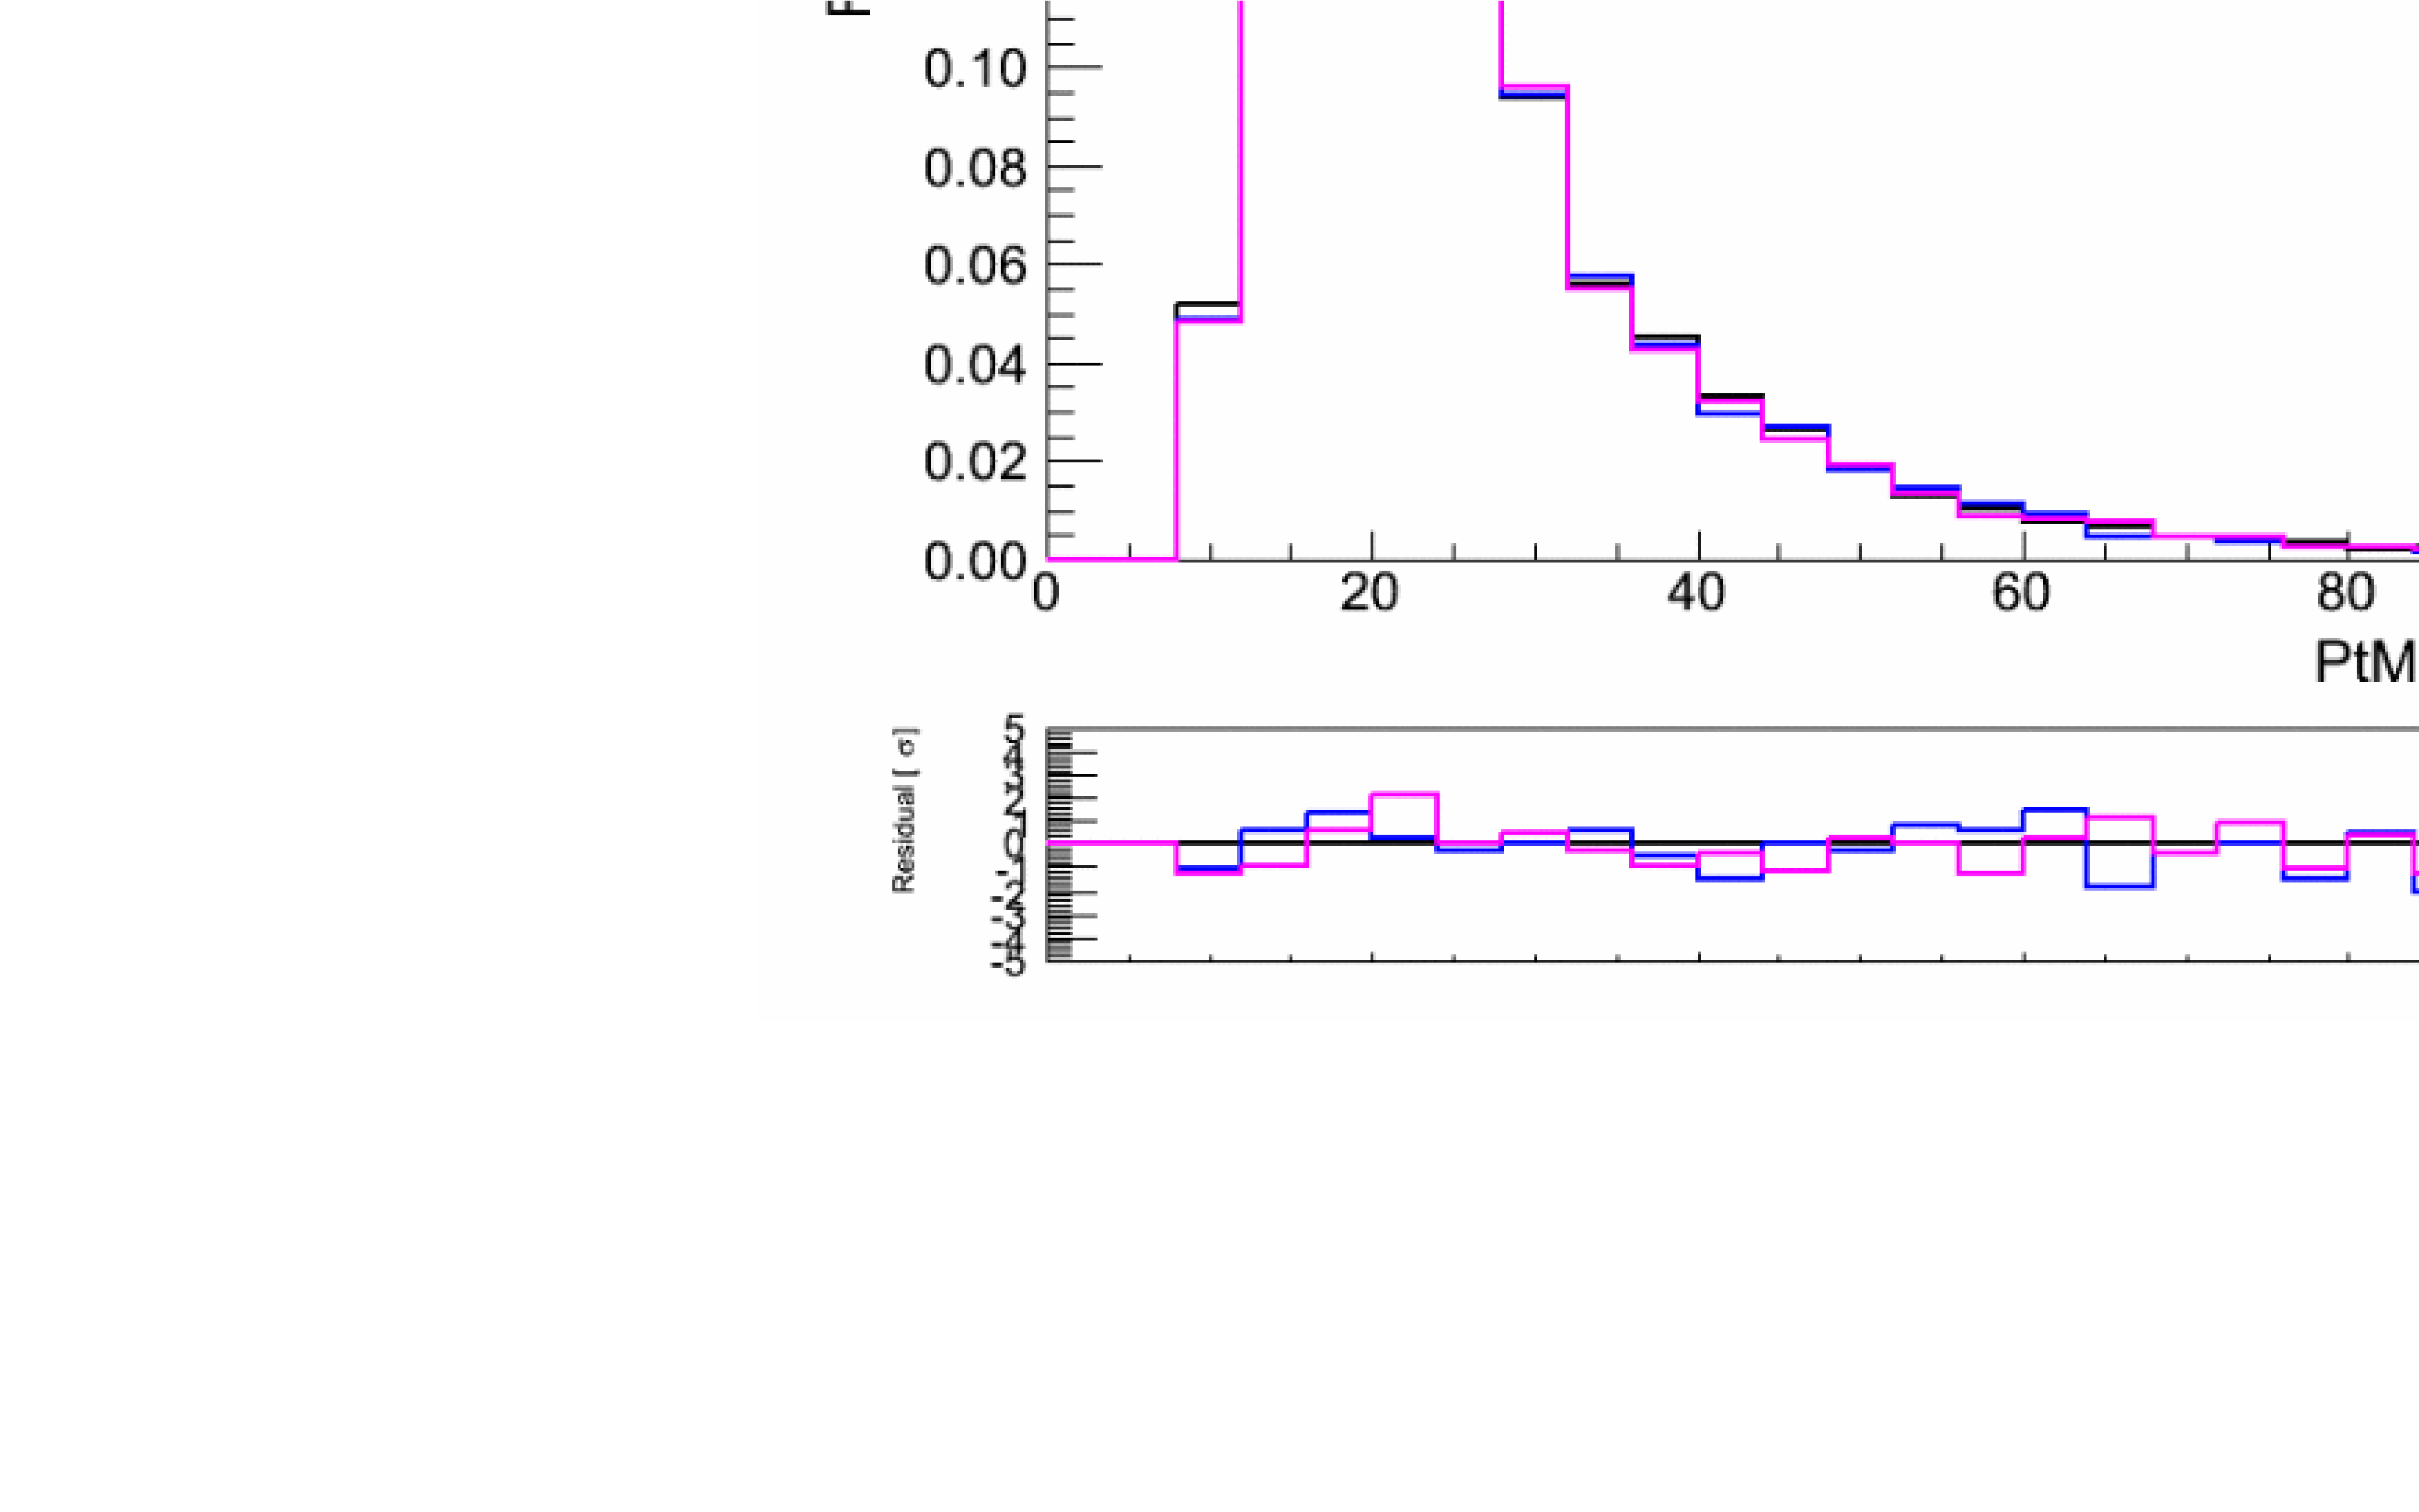
\includegraphics[width=0.49\textwidth]{figures/ShapeSystematics_WW_PtMin.pdf}}
\subfigure[PtMax]{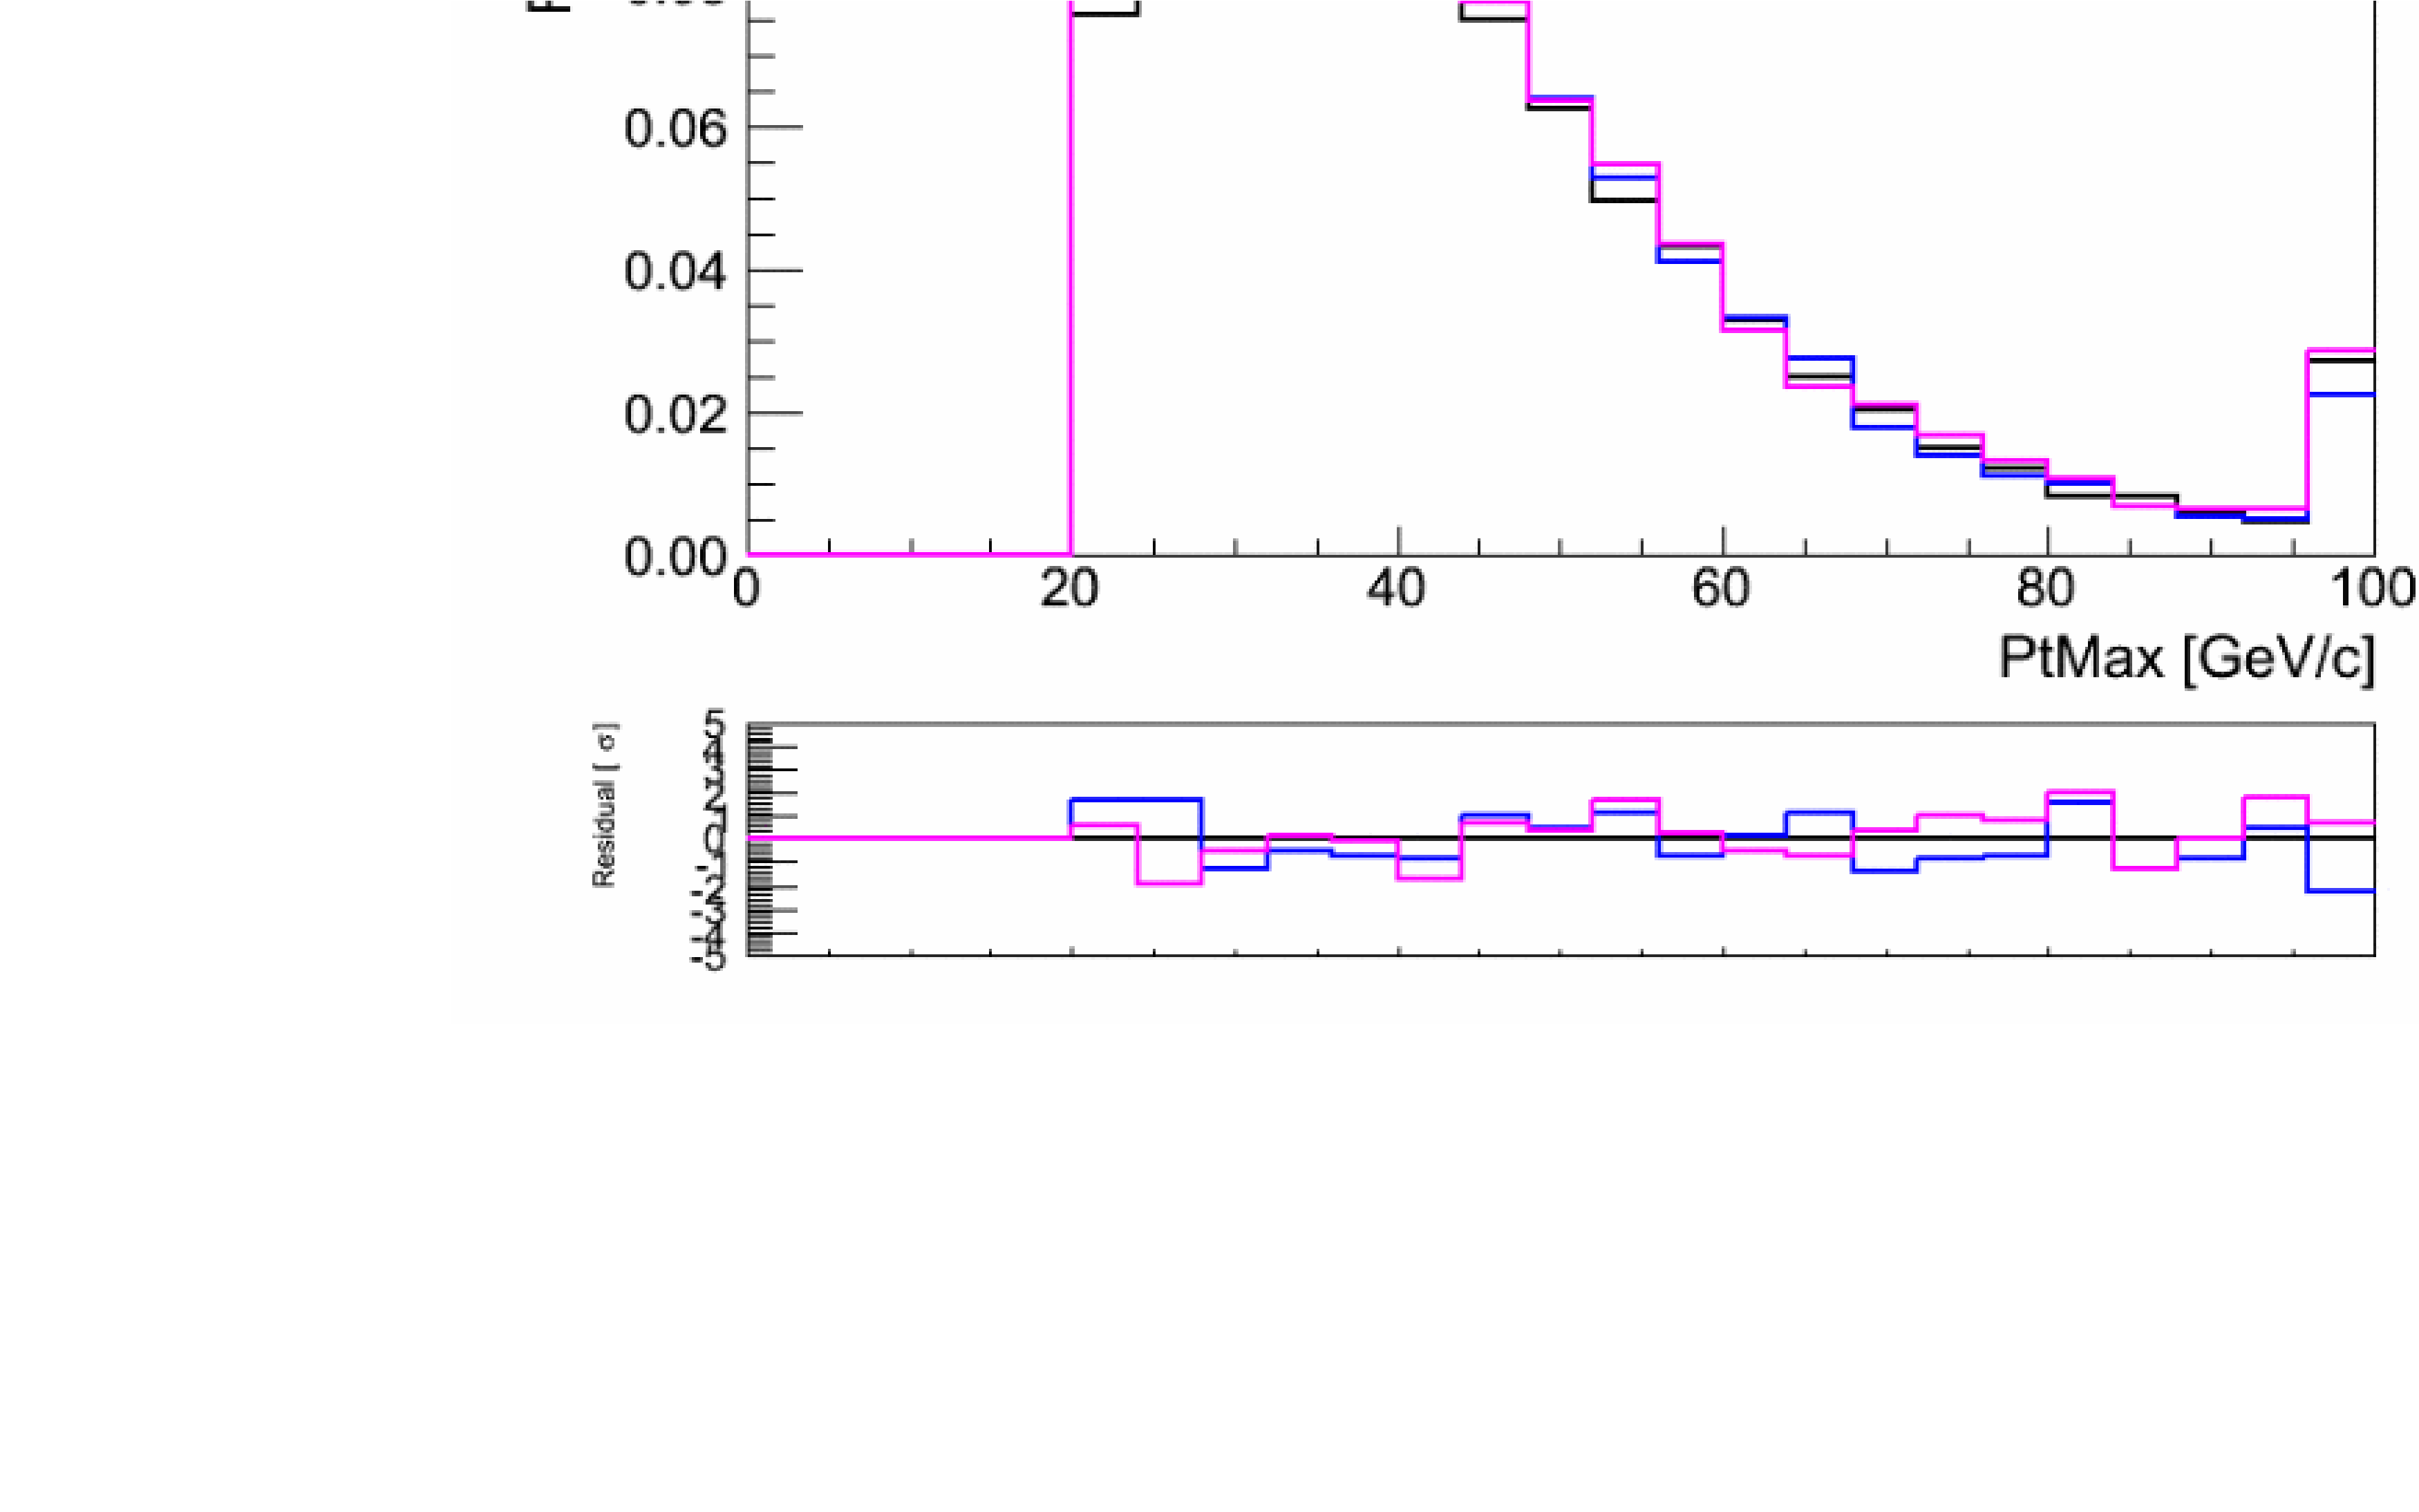
\includegraphics[width=0.49\textwidth]{figures/ShapeSystematics_WW_PtMax.pdf}}
\caption{Comparison of the $p_{T}$ of the leptons for WW background events between the scale 
varied and default predictions from MC@NLO.
}
\label{fig:wwshape_scalevariation_leptonPt}
\end{center}
\end{figure}
%%%%%%%%%%%%%%%%%%%%%%%%%%%%%%%%%%%

%%%%%%%%%%%%%%%%%%%%%%%%%%%%%%%%%%%
\begin{figure}[!htbp]
\begin{center}
\subfigure[$\mathrm{M}_{\mathrm{ll}}$]{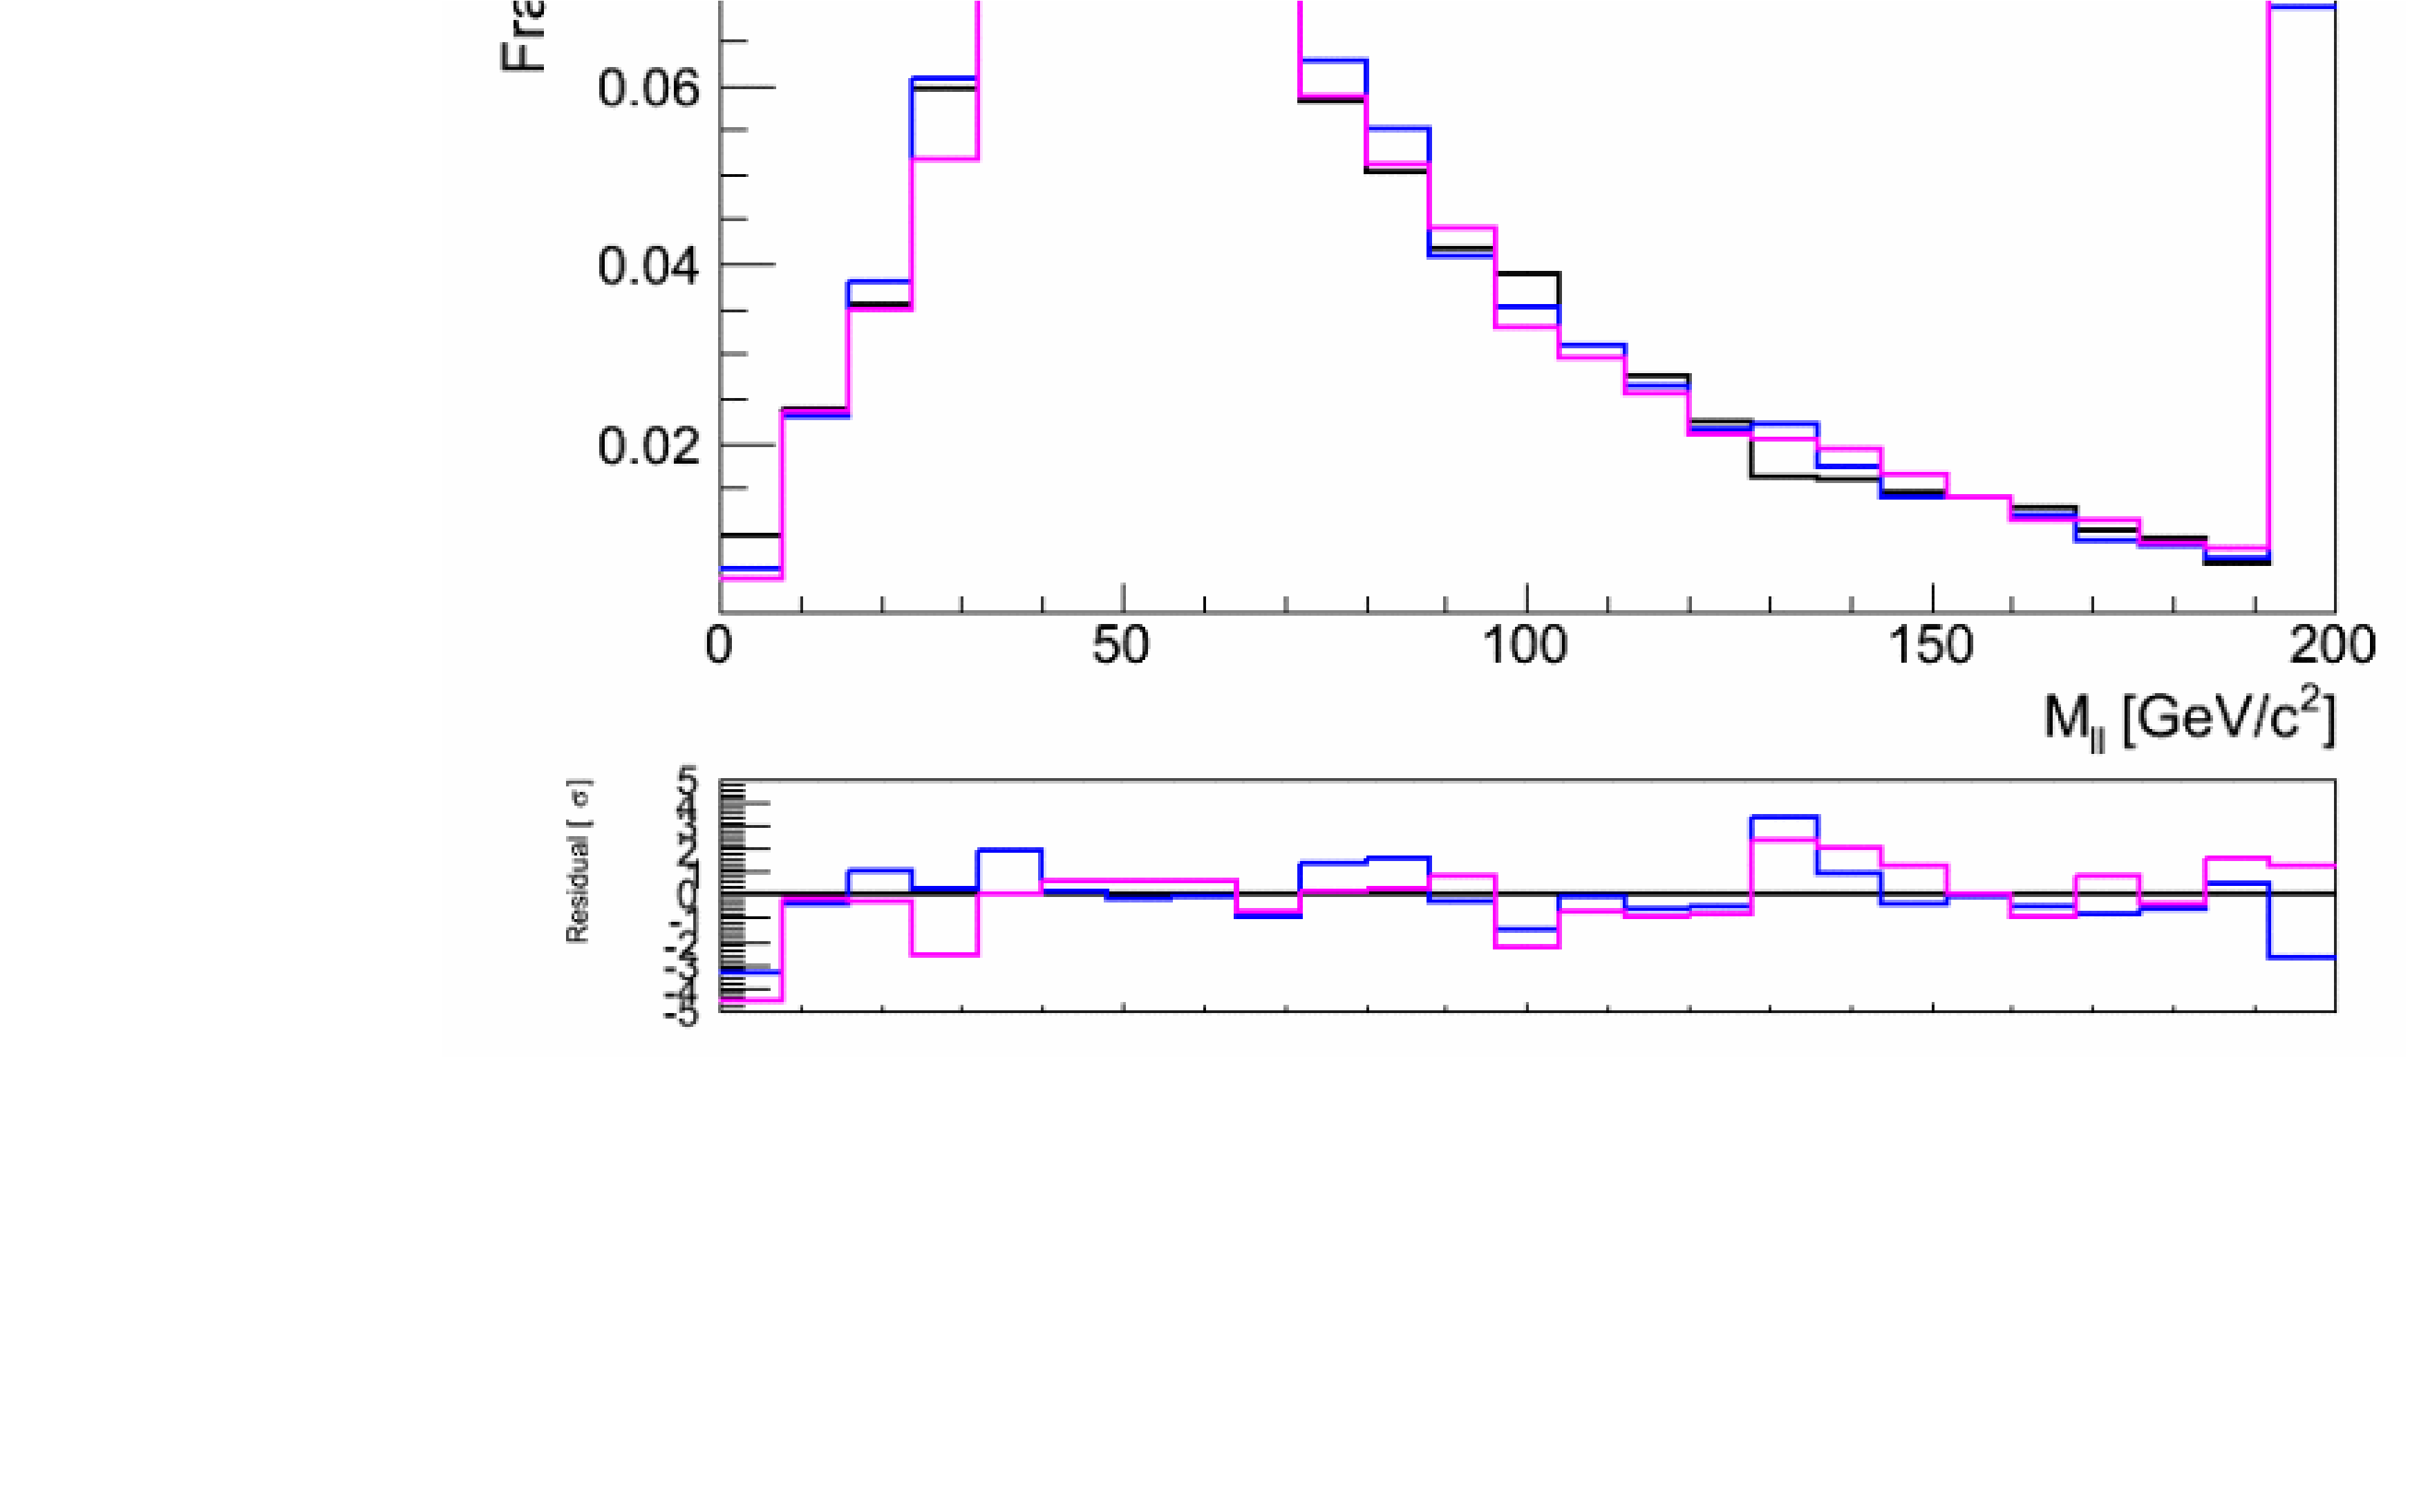
\includegraphics[width=0.49\textwidth]{figures/ShapeSystematics_WW_DileptonMass.pdf}}
\subfigure[$\mathrm{M}_{\mathrm{T}}$]{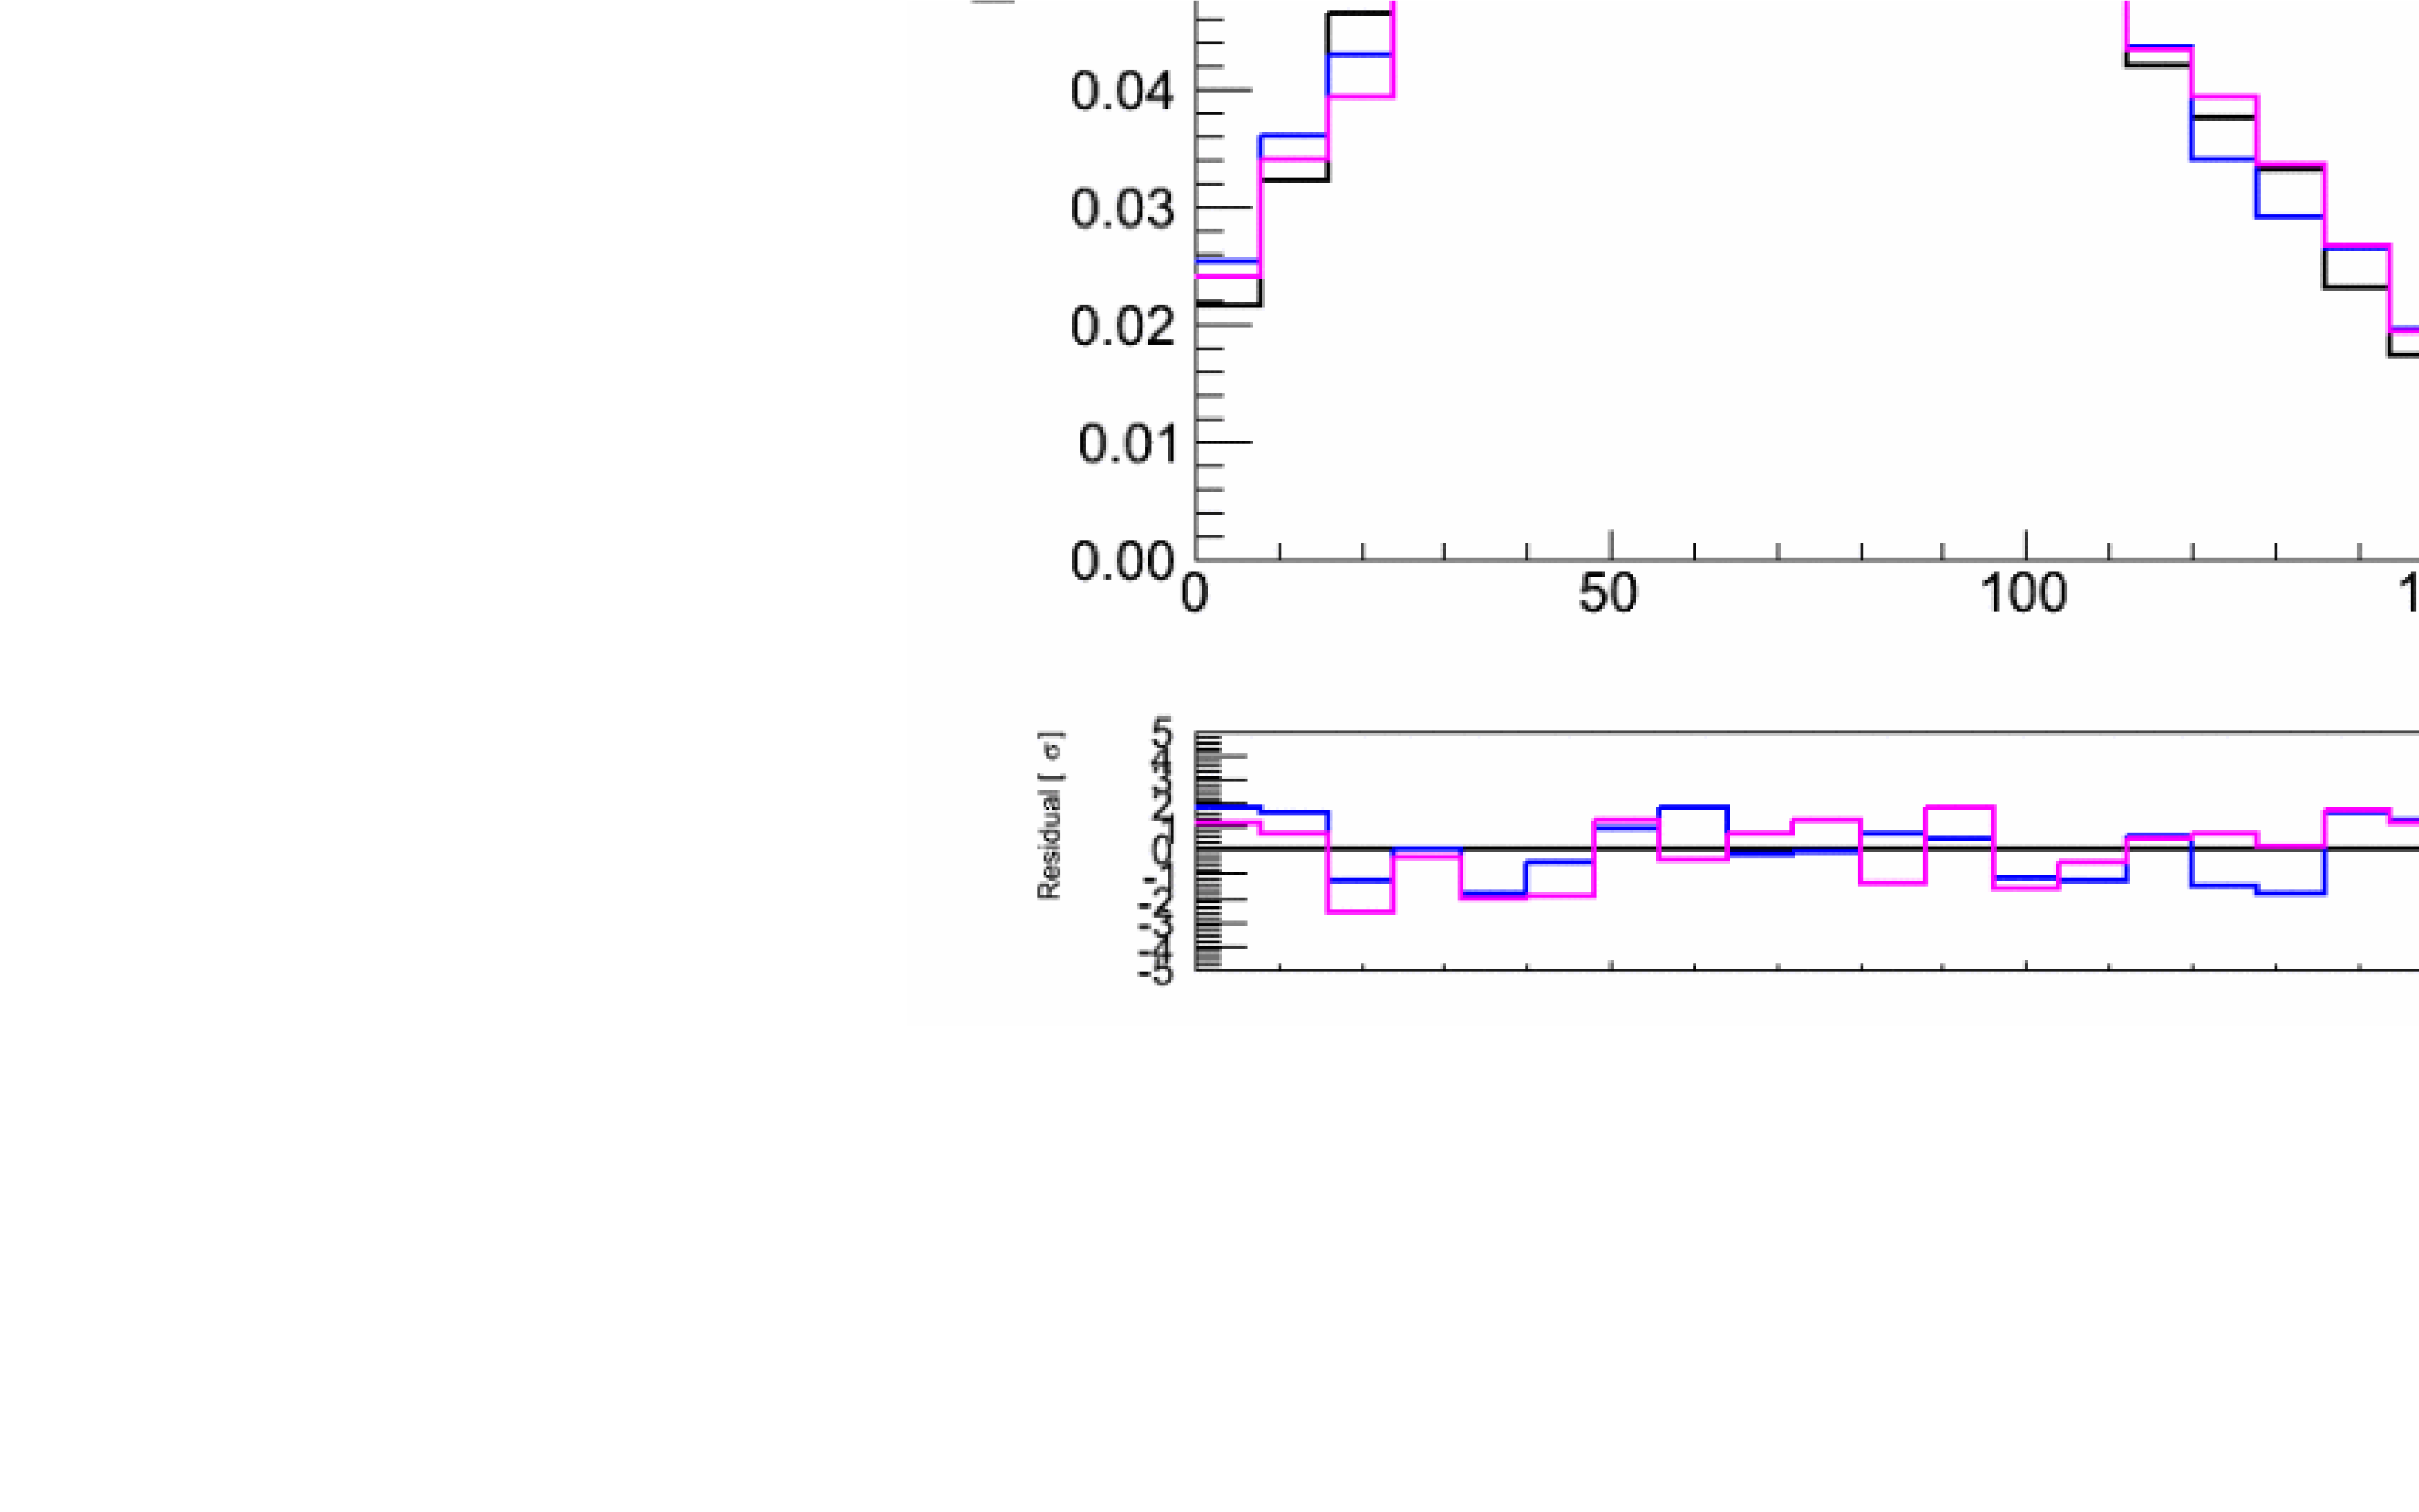
\includegraphics[width=0.49\textwidth]{figures/ShapeSystematics_WW_MTHiggs.pdf}}
\subfigure[$\Delta\phi_{\mathrm{ll}}$]{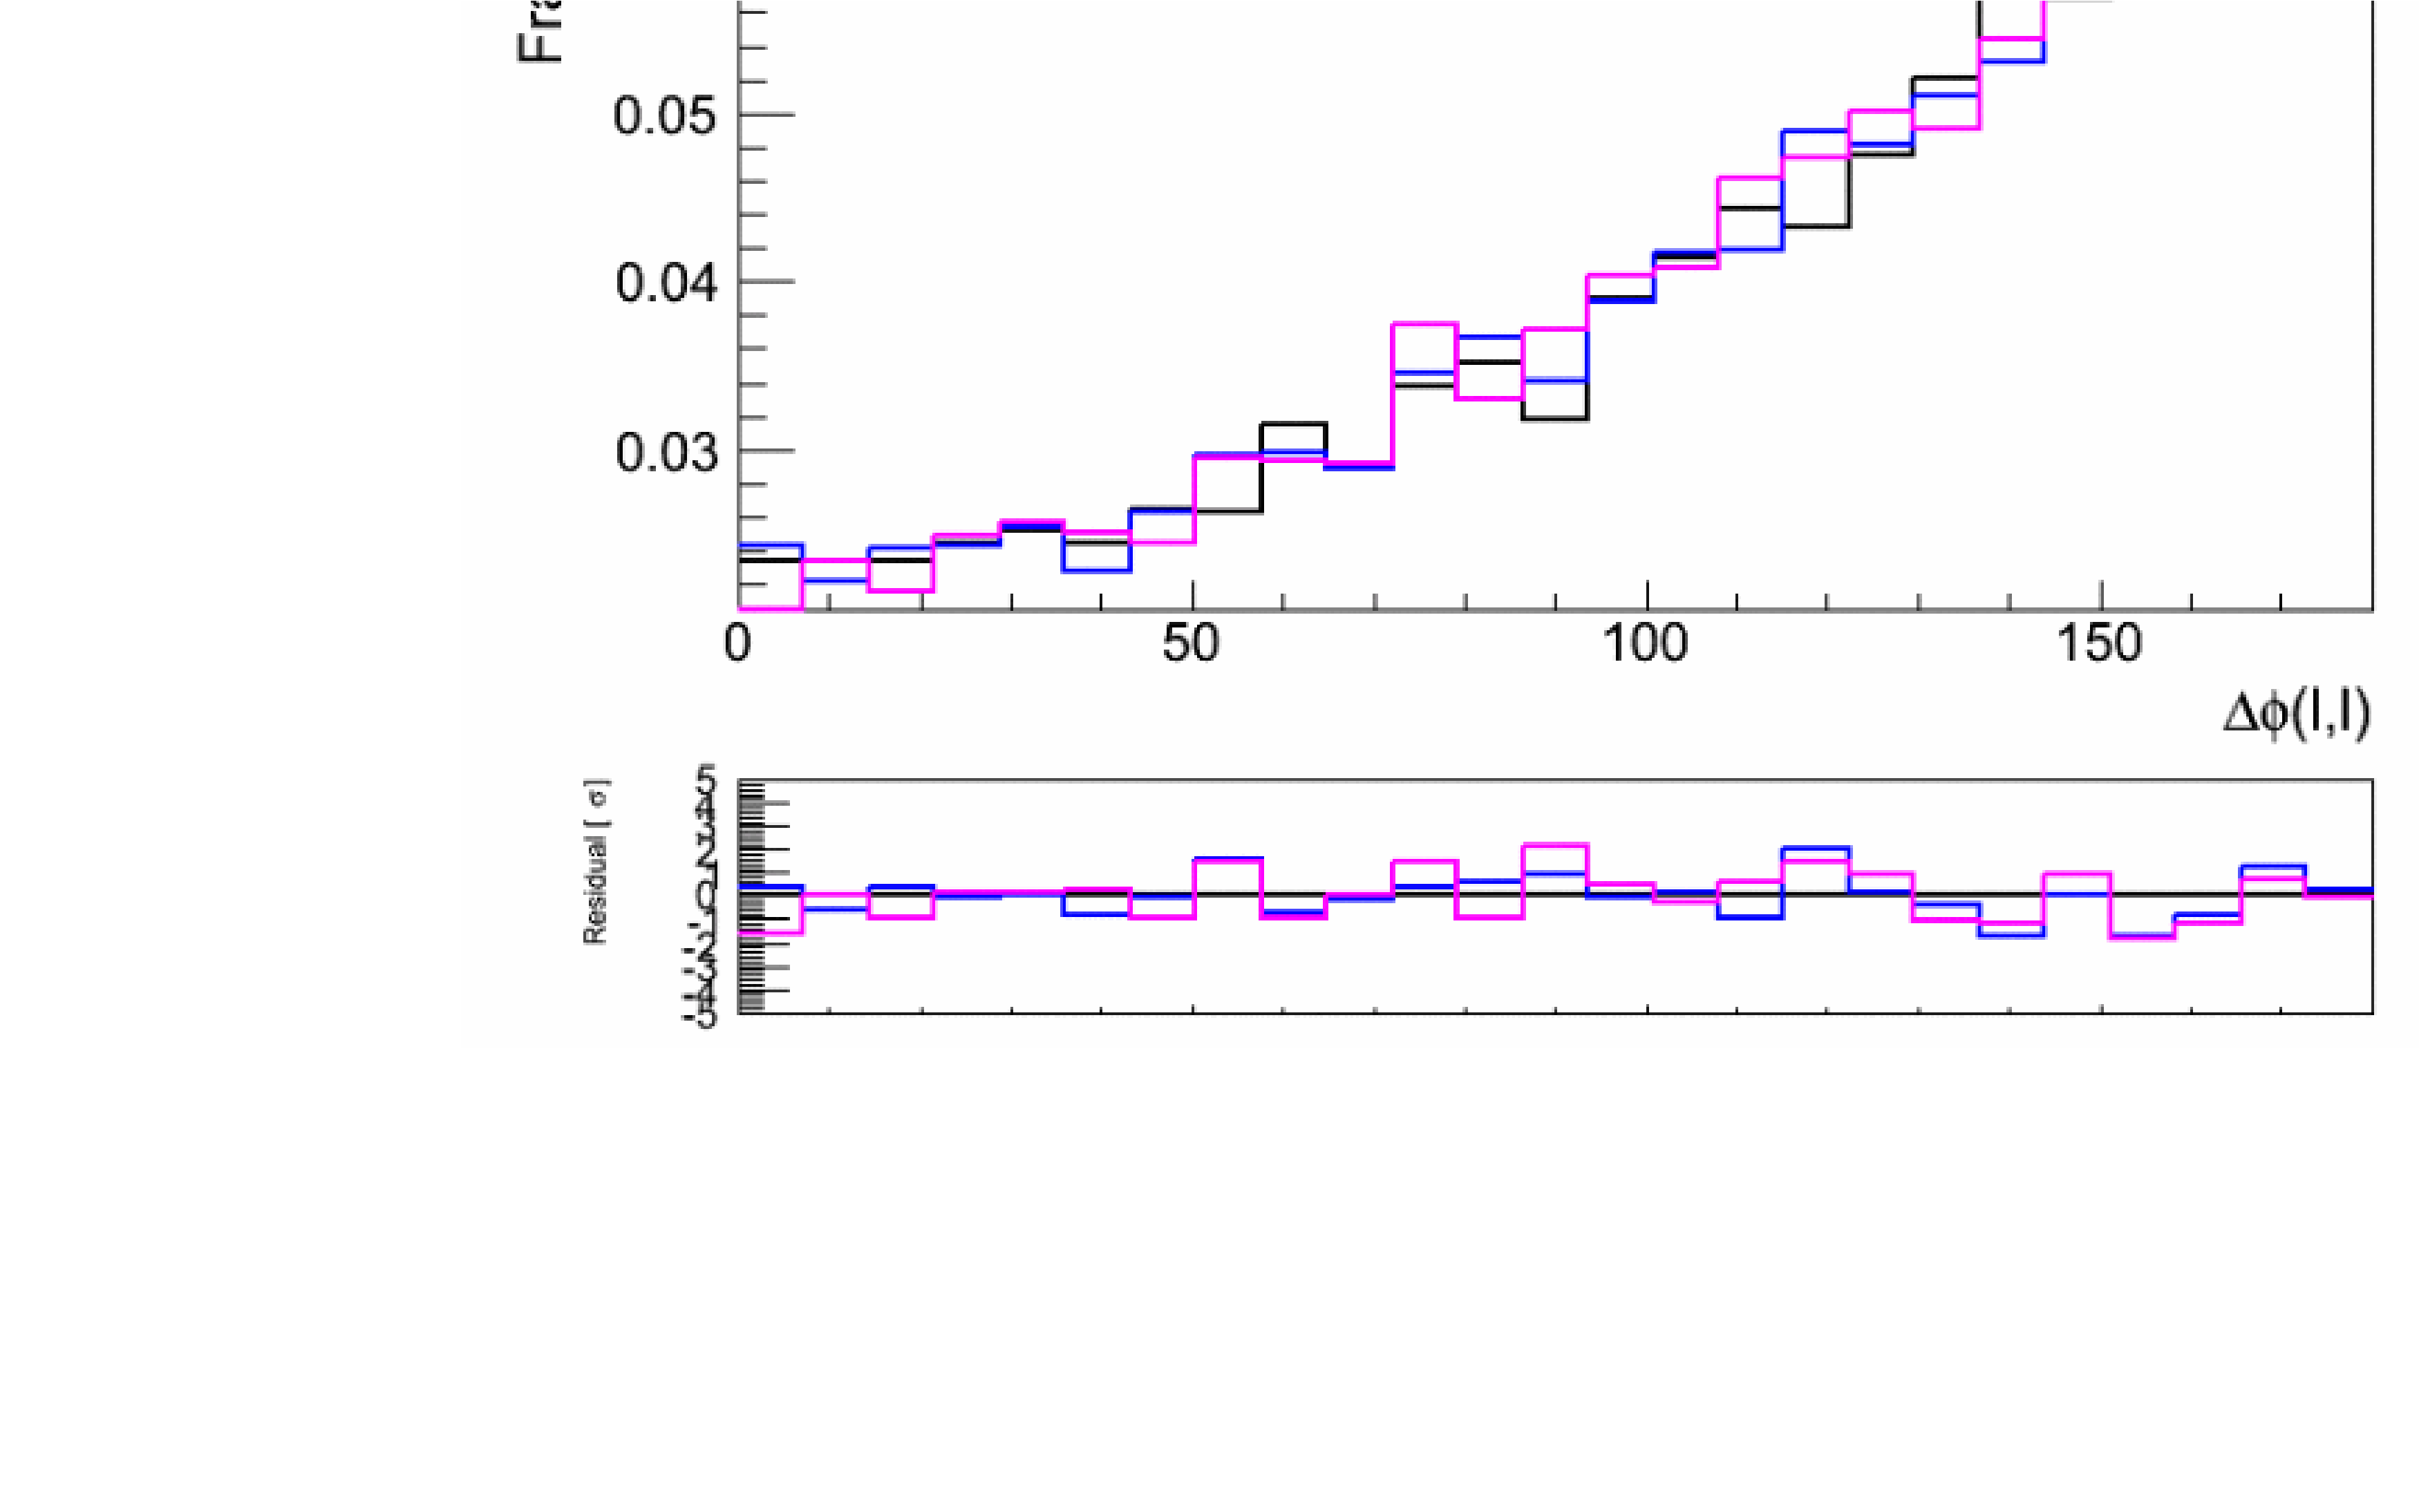
\includegraphics[width=0.49\textwidth]{figures/ShapeSystematics_WW_DeltaPhi.pdf}}
\caption{Comparison of the dilepton mass, the higgs transverse mass, and the $\Delta\phi$ between the 
leptons for WW background events between the scale varied and default predictions from MC@NLO.
}
\label{fig:wwshape_scalevariation_mass}
\end{center}
\end{figure}
%%%%%%%%%%%%%%%%%%%%%%%%%%%%%%%%%%%


In Figure \ref{fig:wwshape_scalevariation_MVA130_MCAtNLO} we show the comparison
of the MVA output distribution trained for the $130$ GeV Higgs mass hypothesis
between the default scale and the up and down scale variation prediction from 
MC@NLO. In Figure \ref{fig:wwshape_scalevariation_MVA130_MadgrahVsMCAtNLO} we
compare the same $M_{H} = 130$GeV MVA output between the scale varied 
MC@NLO predictions and the Madgraph prediction, separately for the 0-Jet
and 1-Jet bins. Finally, the analogous comparison is made in Figure 
\ref{fig:wwshape_scalevariation_MVA300_MadgrahVsMCAtNLO} for the MVA
output trained for the $300$ GeV Higgs mass hypothesis. 



%%%%%%%%%%%%%%%%%%%%%%%%%%%%%%%%%%%
\begin{figure}[!htbp]
\begin{center}
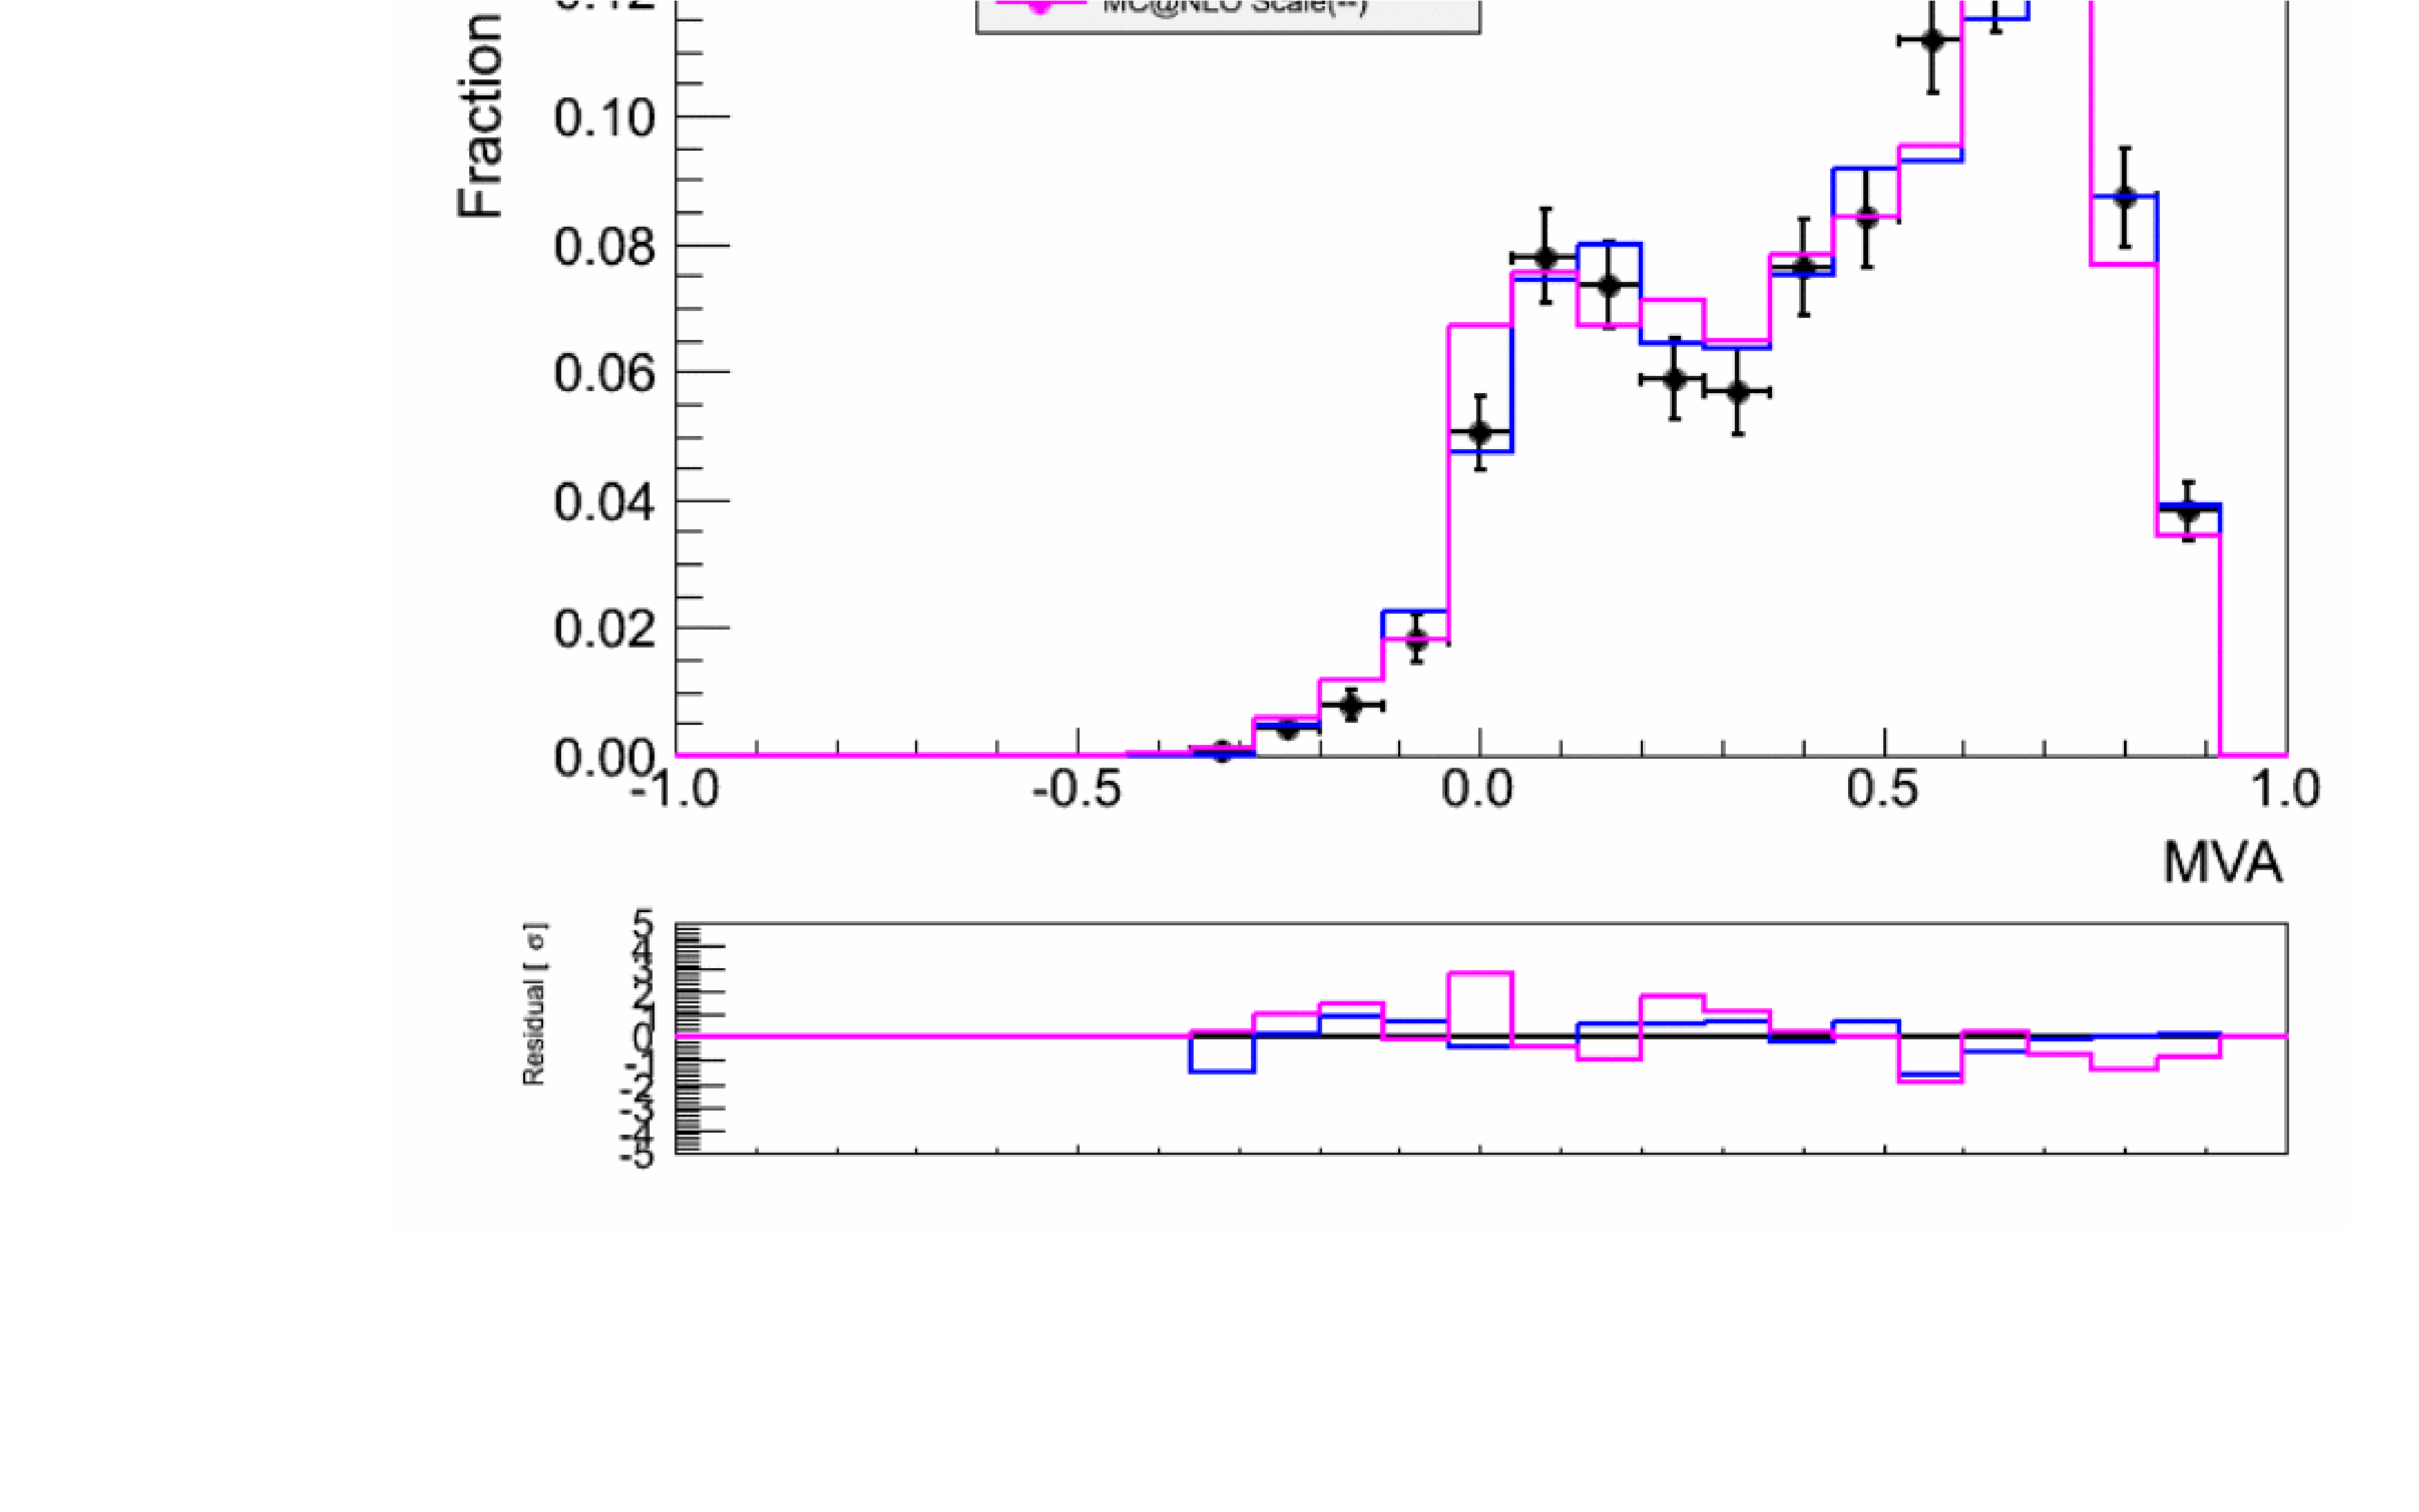
\includegraphics[width=0.49\textwidth]{figures/ShapeSystematics_WW0JetBin_MVA130_MCAtNLOScaleVariation.pdf}
\caption{Comparison of the MVA output trained on the $M_{H}=130$ GeV Higgs mass hypothesis 
for WW background events between the scale varied and default predictions from MC@NLO.
}
\label{fig:wwshape_scalevariation_MVA130_MCAtNLO}
\end{center}
\end{figure}
%%%%%%%%%%%%%%%%%%%%%%%%%%%%%%%%%%%

%%%%%%%%%%%%%%%%%%%%%%%%%%%%%%%%%%%
\begin{figure}[!htbp]
\begin{center}
\subfigure[mH=130 0-Jet MVA]{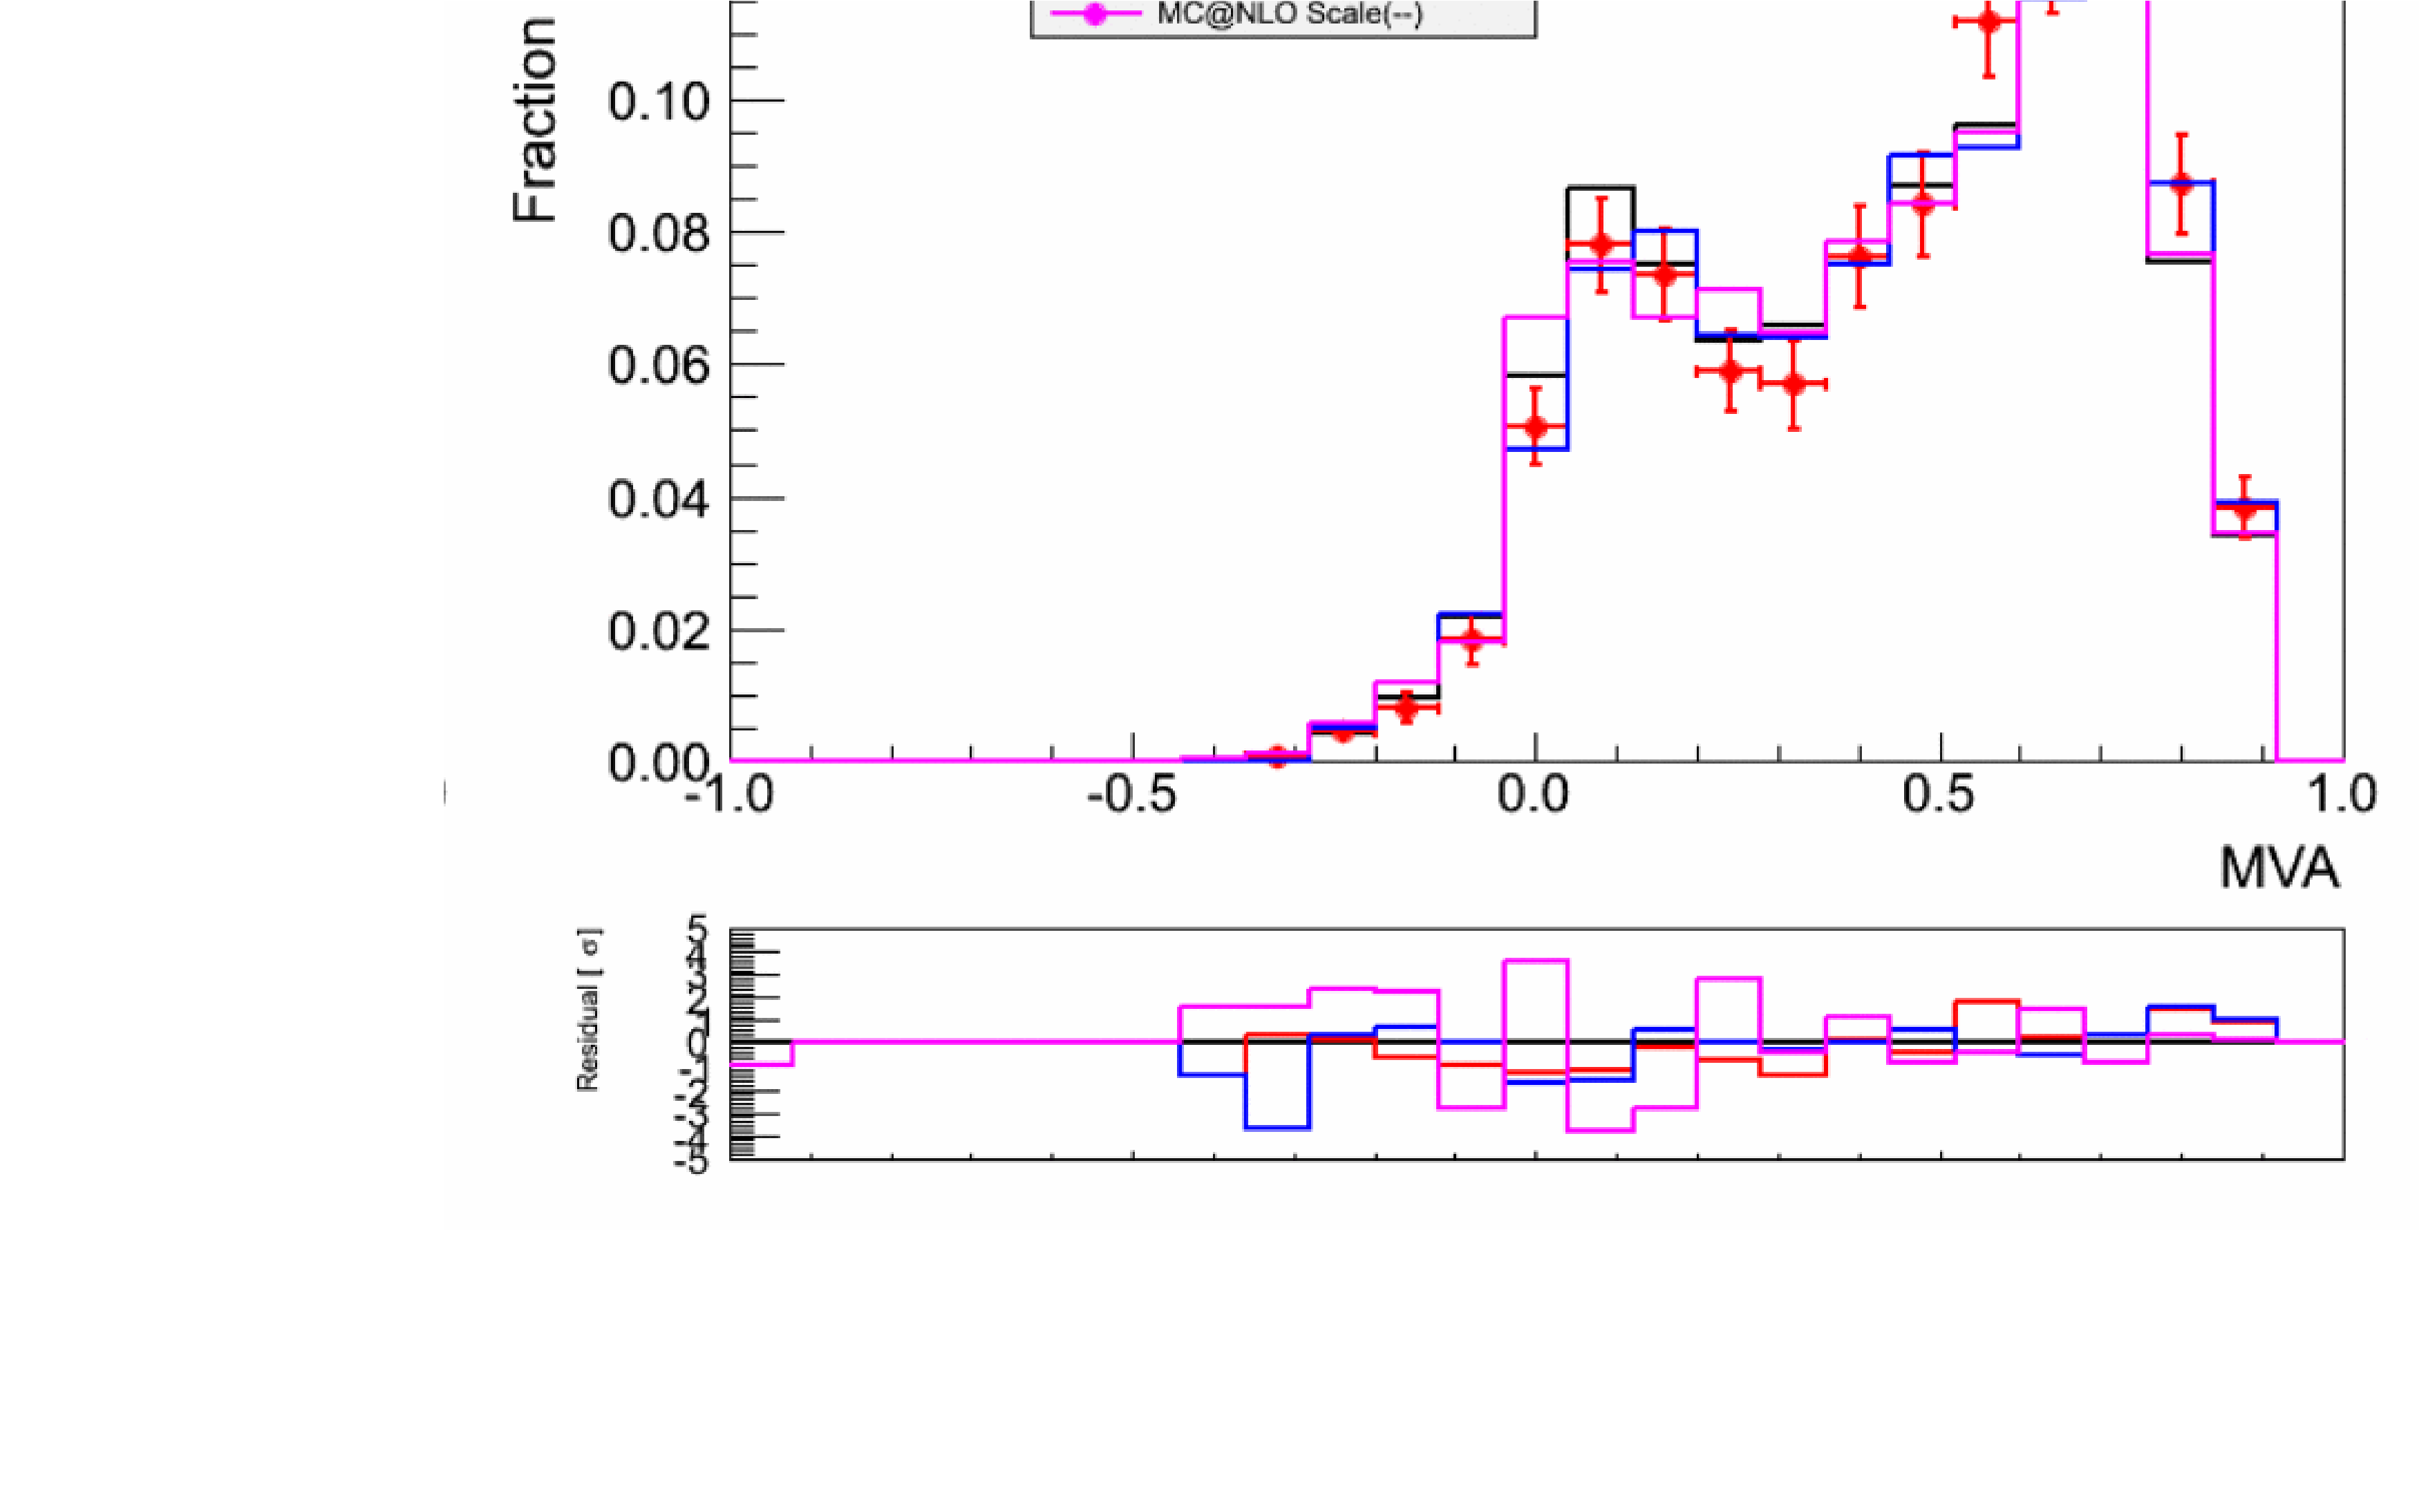
\includegraphics[width=0.49\textwidth]{figures/ShapeSystematics_WW0JetBin_MVA130_MadgraphVsMCAtNLO.pdf}}
\subfigure[mH=130 1-Jet MVA]{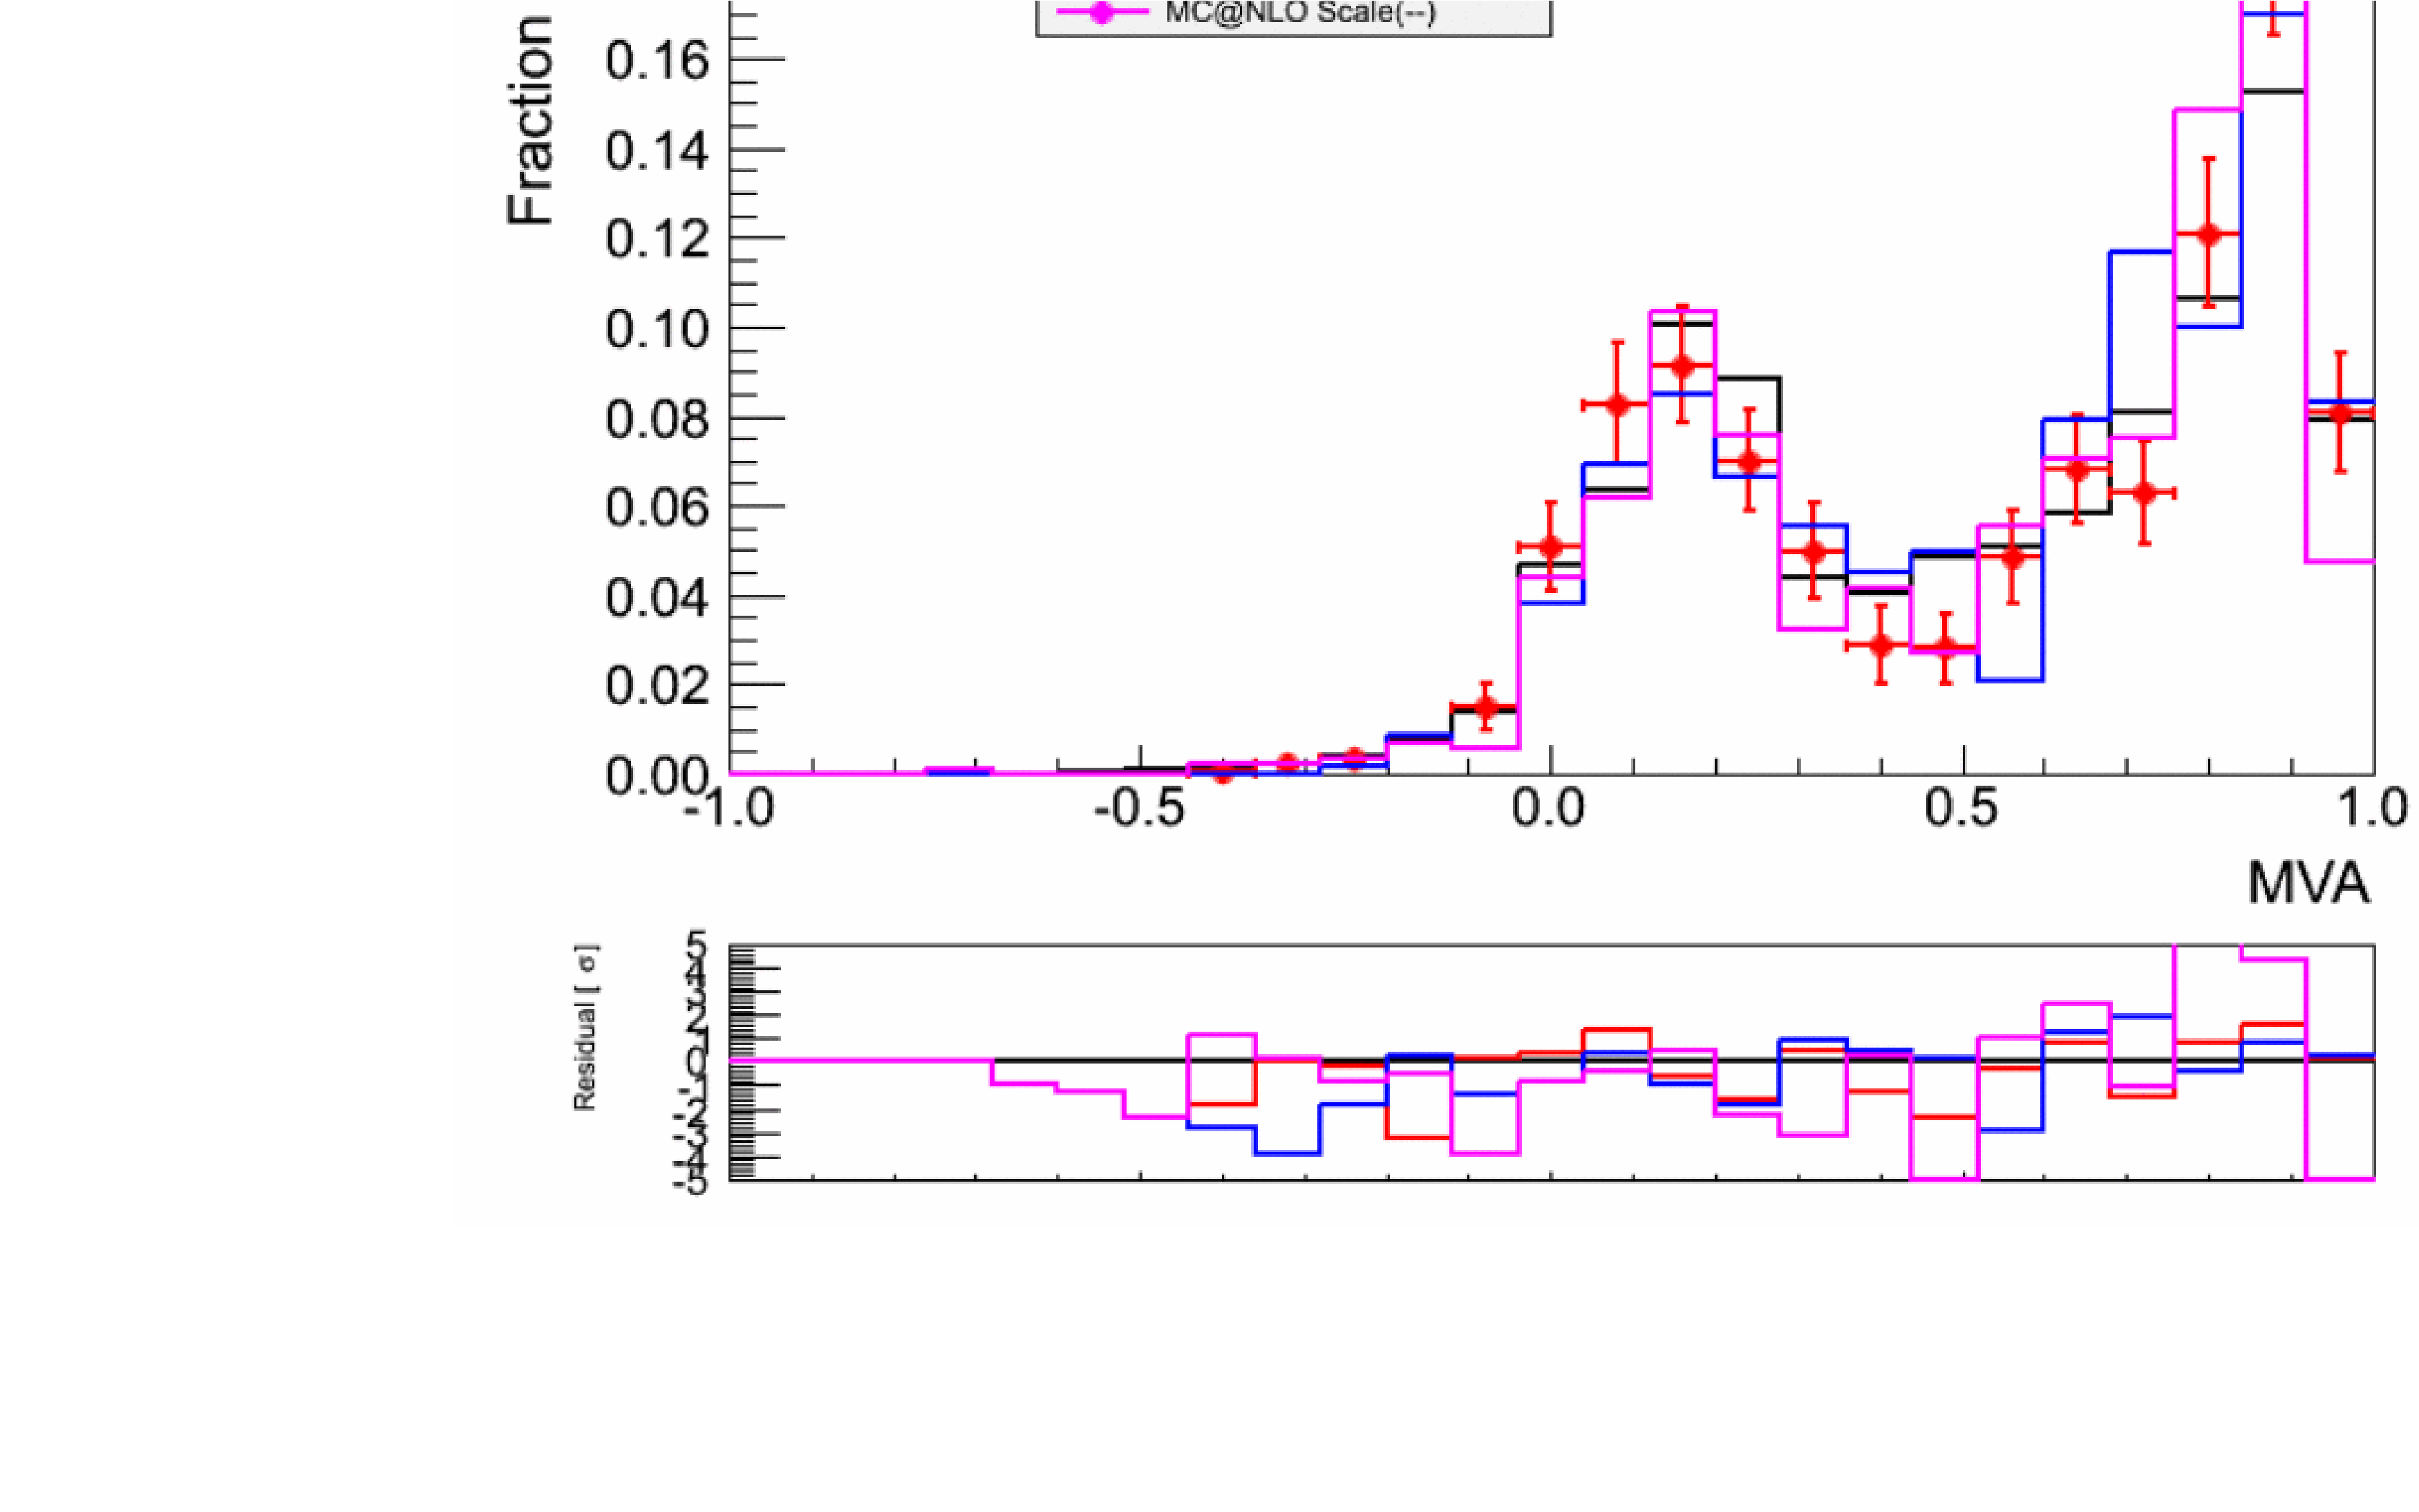
\includegraphics[width=0.49\textwidth]{figures/ShapeSystematics_WW1JetBin_MVA130_MadgraphVsMCAtNLO.pdf}}
\caption{Comparison of the MVA output trained on the $M_{H}=130$ GeV Higgs mass hypothesis
for WW background events between the scale varied and default predictions from MC@NLO,
separately for the 0-Jet and 1-Jet bins.
}
\label{fig:wwshape_scalevariation_MVA130_MadgrahVsMCAtNLO}
\end{center}
\end{figure}
%%%%%%%%%%%%%%%%%%%%%%%%%%%%%%%%%%%

%%%%%%%%%%%%%%%%%%%%%%%%%%%%%%%%%%%
\begin{figure}[!htbp]
\begin{center}
\subfigure[mH=300 0-Jet MVA]{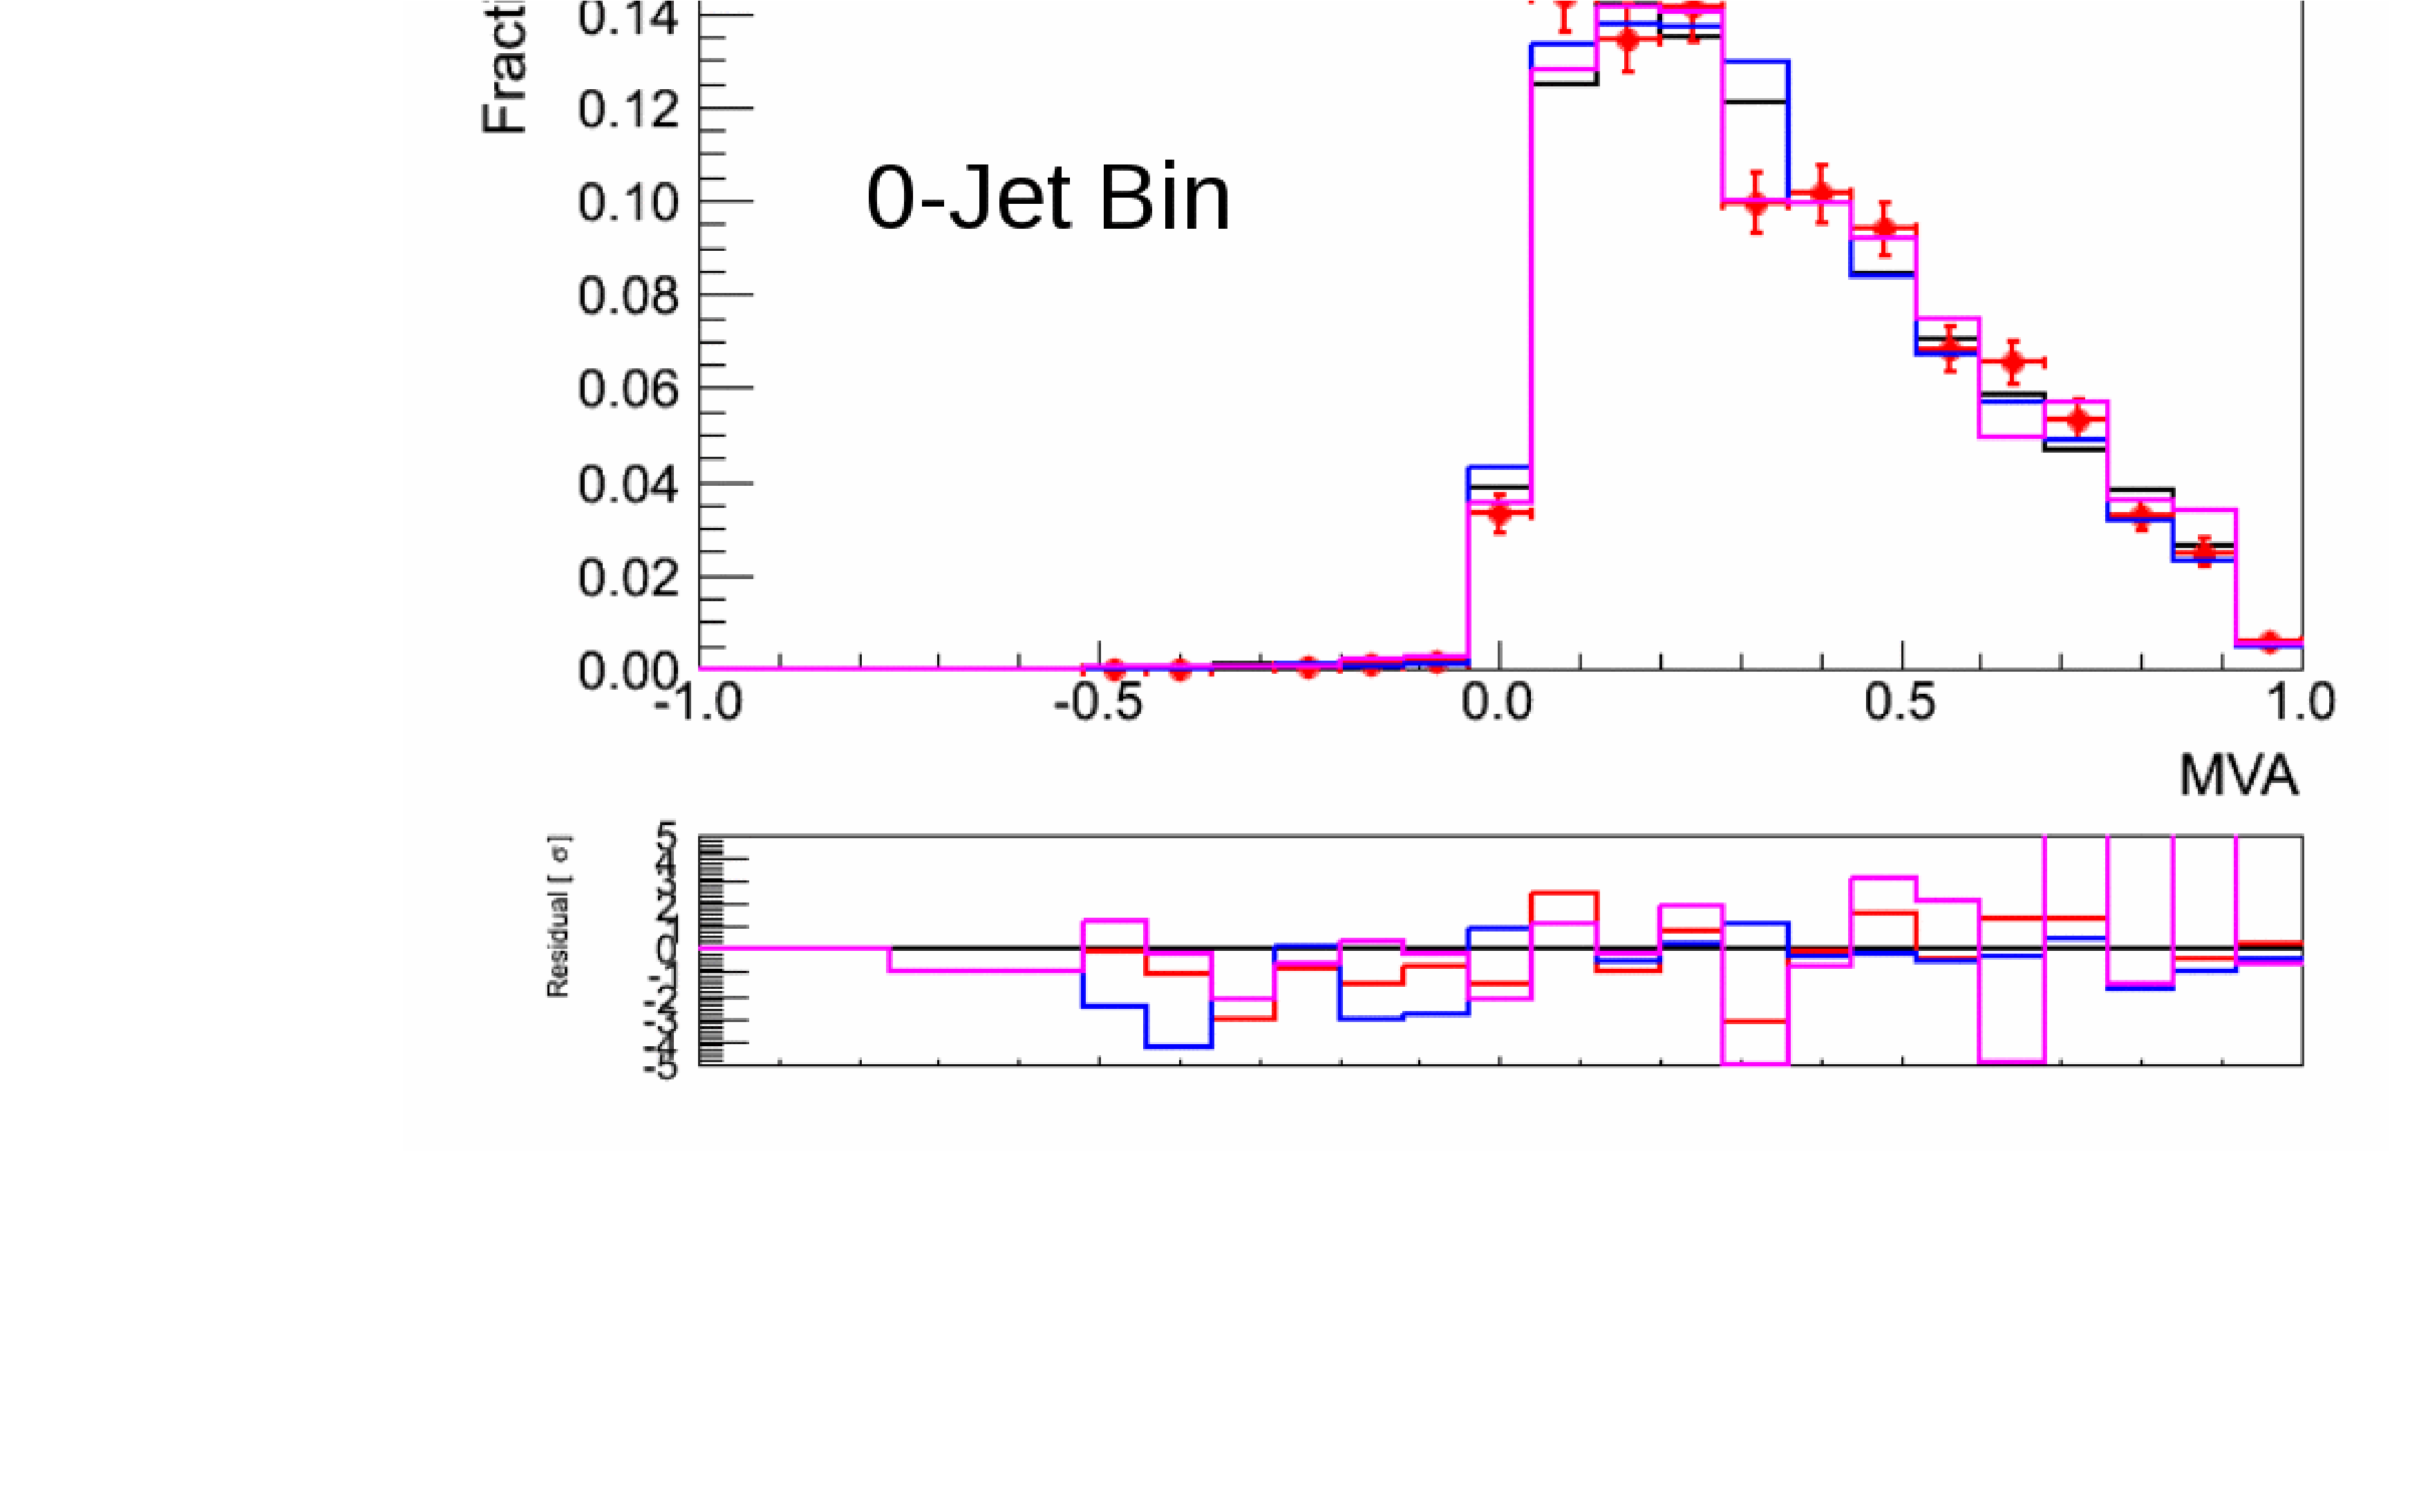
\includegraphics[width=0.49\textwidth]{figures/ShapeSystematics_WW0JetBin_MVA300_MadgraphVsMCAtNLO.pdf}}
\subfigure[mH=300 1-Jet MVA]{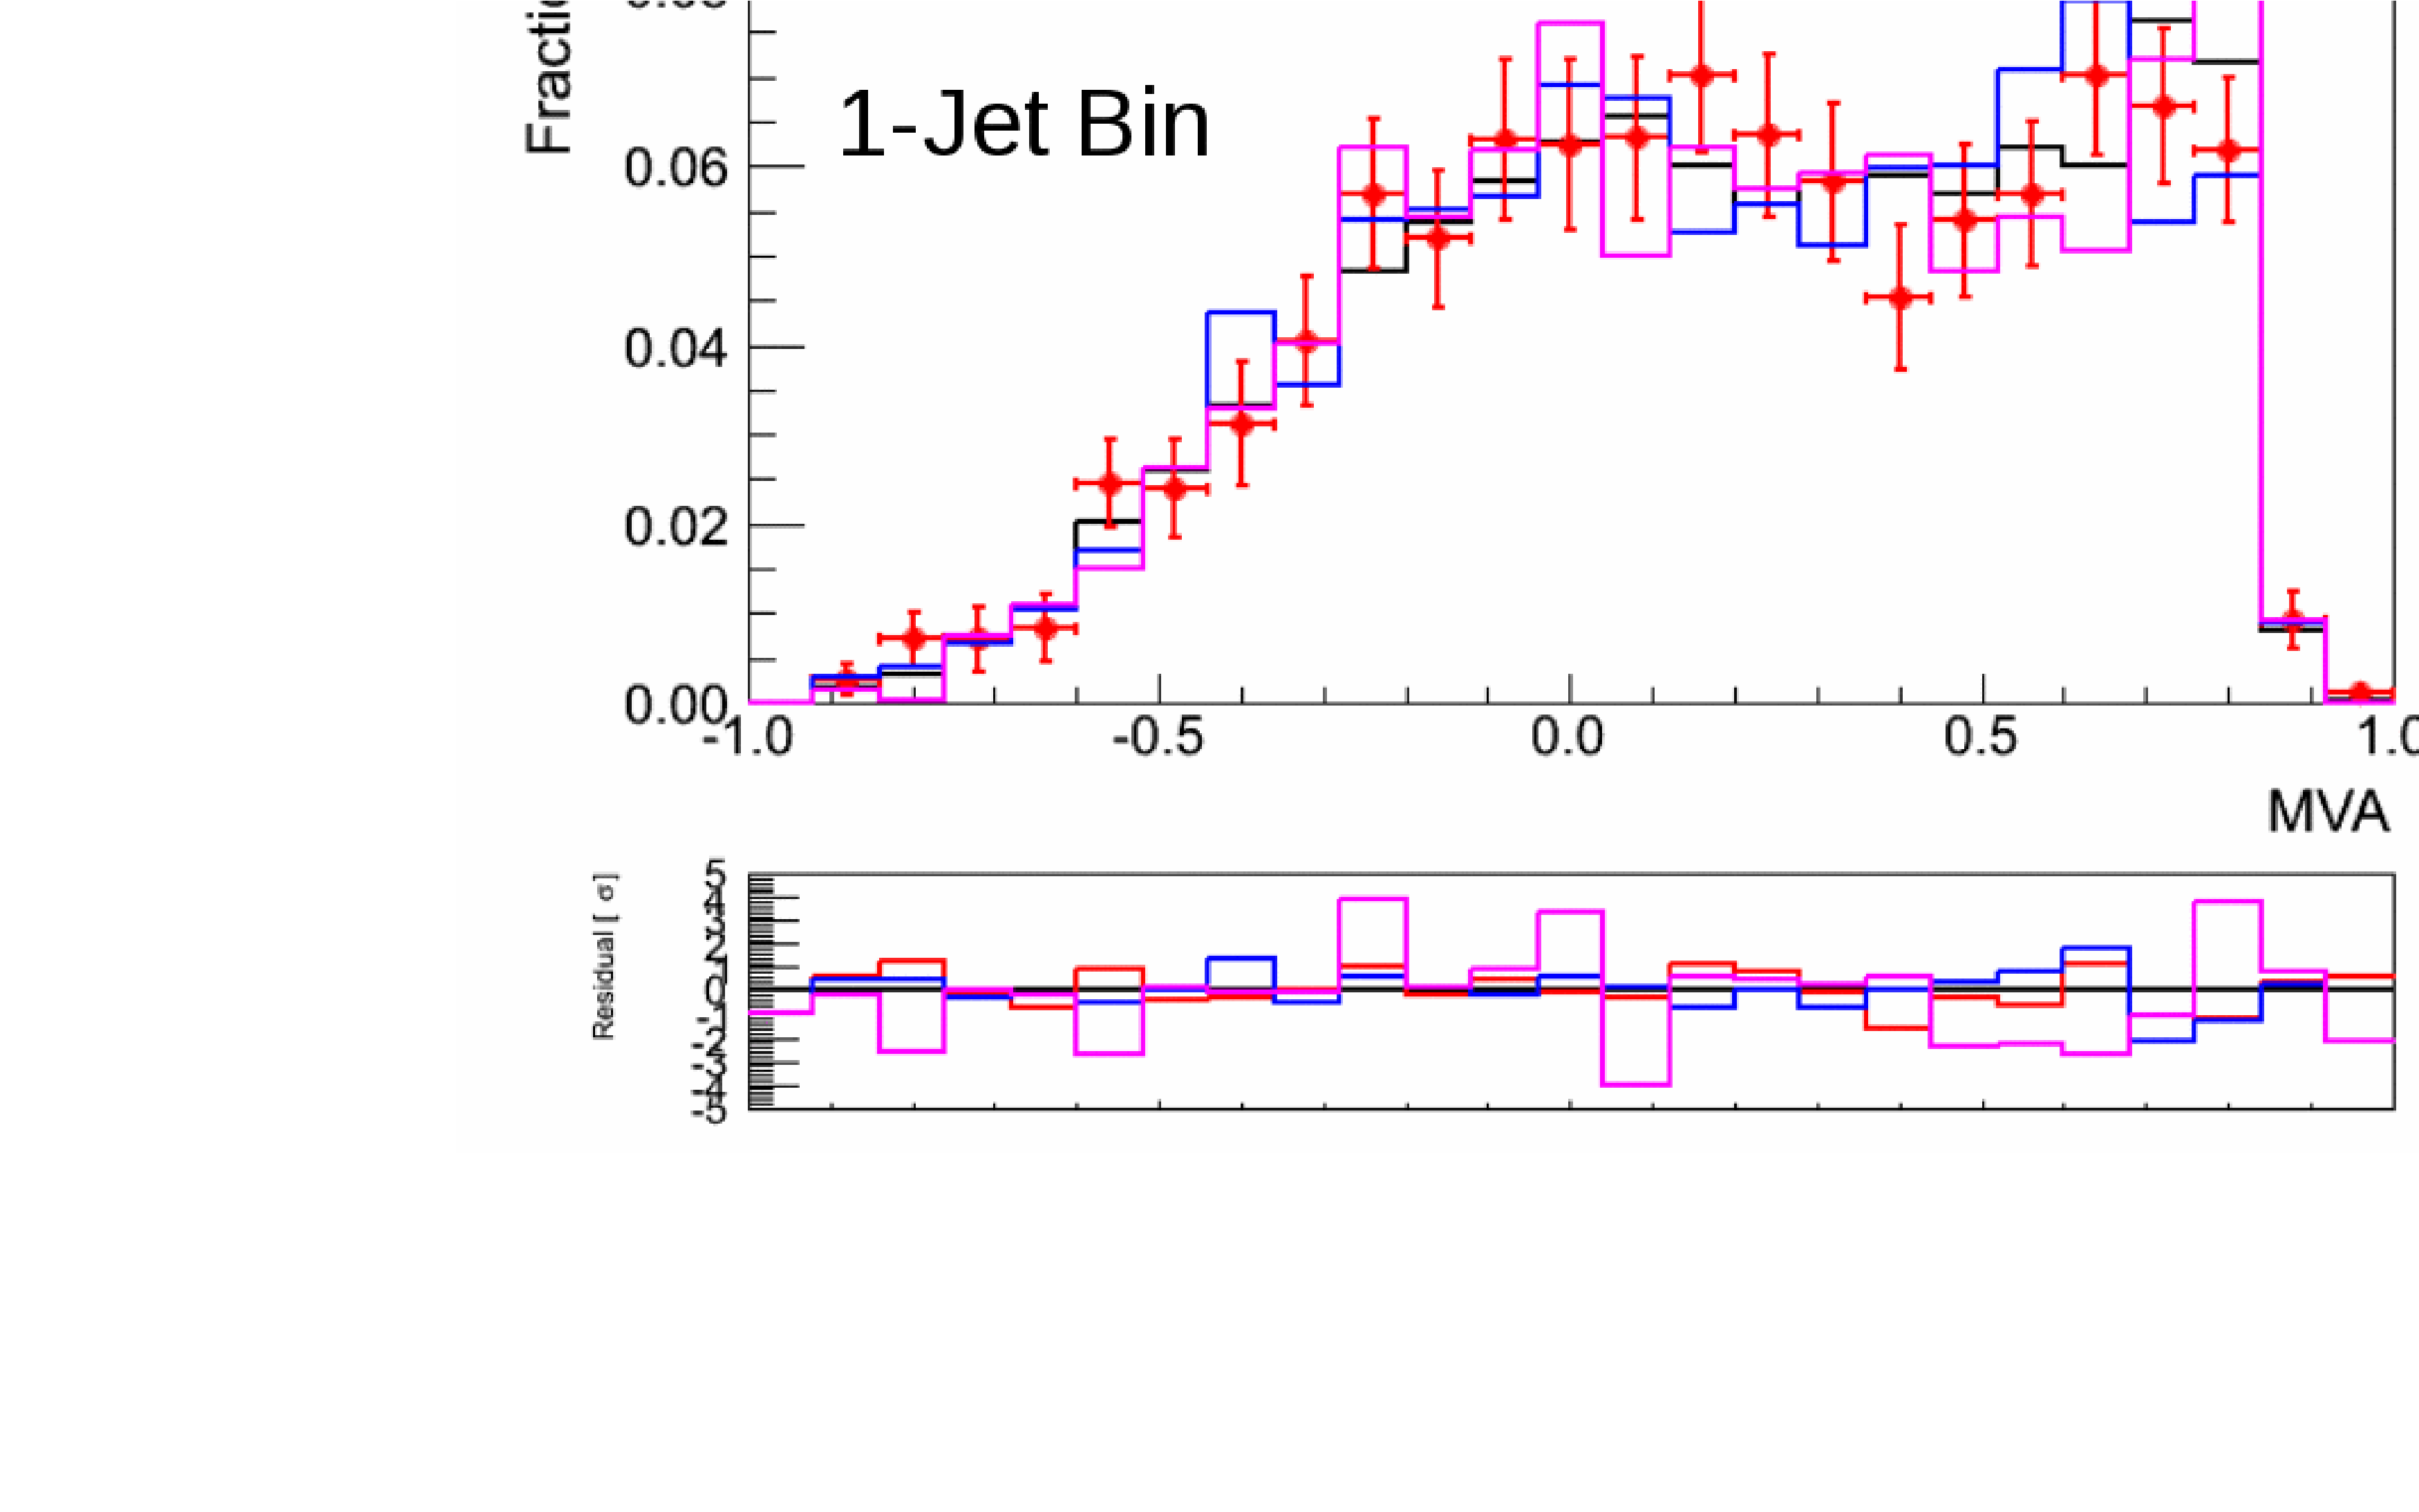
\includegraphics[width=0.49\textwidth]{figures/ShapeSystematics_WW1JetBin_MVA300_MadgraphVsMCAtNLO.pdf}}
\caption{Comparison of the MVA output trained on the $M_{H}=300$ GeV Higgs mass hypothesis
for WW background events between the scale varied and default predictions from MC@NLO,
separately for the 0-Jet and 1-Jet bins.
}
\label{fig:wwshape_scalevariation_MVA300_MadgrahVsMCAtNLO}
\end{center}
\end{figure}
%%%%%%%%%%%%%%%%%%%%%%%%%%%%%%%%%%%

In summary, we do not observe any significant differences among the different 
Monte Carlo predictions beyond statistical uncertainties of the Monte Carlo
sample.
